\documentclass[a4paper,11pt,final]{article}
% Pour une impression recto verso, utilisez plutôt ce documentclass :
%\documentclass[a4paper,11pt,twoside,final]{article}

\usepackage[english,francais]{babel}
\usepackage[normalem]{ulem}
\usepackage[utf8]{inputenc}
\usepackage[T1]{fontenc}
\usepackage[pdftex]{graphicx}
\usepackage{setspace}
\usepackage{hyperref}
% \usepackage[french]{varioref}
\usepackage{amsmath}
\usepackage{mathtools}
\usepackage{systeme}
\usepackage{amssymb}
\usepackage[usenames,dvipsnames]{color}
\usepackage[usenames,dvipsnames,svgnames,table]{xcolor}
\usepackage{cancel} % needed by: 9
\usepackage{framed}
\usepackage{array}
%\usepackage{enumitem} % needed by: 17
\usepackage{lmodern} % needed by: 17
\usepackage{listings} % needed by: 17
\usepackage{color} % needed by: 17
\usepackage{tikz} % needed by: 17
\usepackage{array} % needed by: 17

\definecolor{mygreen}{rgb}{0,0.6,0} % needed by: 17
\definecolor{mygray}{rgb}{0.5,0.5,0.5} % needed by: 17
\definecolor{mymauve}{rgb}{0.58,0,0.82} % needed by: 17

\selectlanguage{french}

\DeclareUnicodeCharacter{22A8}{\tautologie}
\DeclareUnicodeCharacter{22AD}{\contradiction}

\newcommand{\reporttitle}{LINGI1101\\
\vspace{\baselineskip}
Logique et Structures Discrètes}     % Titre
\newcommand{\reportauthor}{Peter \textsc{Van Roy}} % Auteur
\newcommand{\reportsubject}{ } % Sujet
\newcommand{\HRule}{\rule{\linewidth}{0.5mm}}
\setlength{\parskip}{1ex} % Espace entre les paragraphes

\newcommand{\true}{\mathrm{true}}
\newcommand{\false}{\mathrm{false}}
\newcommand{\val}{\mathrm{val}}
\newcommand{\VAL}{\mathrm{VAL}}

\hypersetup{
    pdftitle={\reporttitle},%
    pdfauthor={\reportauthor},%
    pdfsubject={\reportsubject},%
    pdfkeywords={rapport} {vos} {mots} {clés}
}

\begin{document}
  % Inspiré de http://en.wikibooks.org/wiki/LaTeX/Title_Creation

\begin{titlepage}

\begin{center}

\begin{minipage}[t]{0.8\textwidth}
  \begin{center}
    
\includegraphics [width=70mm]{images/logo_Ucl.jpg} \\[0.5cm]
    % \begin{spacing}{1.5}
    %   \textsc{\LARGE Université catholique de Louvain}
    % \end{spacing}
  \end{center}
\end{minipage}
% \begin{minipage}[t]{0.48\textwidth}
%   \begin{flushright}
%     
\includegraphics [width=30mm]{images/logo-societe.jpg} \\[0.5cm]
%     \textsc{\LARGE Entreprise}
%   \end{flushright}
% \end{minipage} \\[1.5cm]

\textsc{\Large \reportsubject}\\[0.5cm]
\HRule \\[0.4cm]
{\huge \bfseries \reporttitle}\\[0.4cm]
\HRule \\[1.5cm]

\begin{minipage}[t]{0.5\textwidth}
  \begin{center} \large
    \emph{Titulaire:} \reportauthor
  \end{center}
\end{minipage}
% \begin{minipage}[t]{0.6\textwidth}
%   \begin{flushright} \large
%     \emph{Responsables :} \\
%     M.~Jean \textsc{Machin} \\
%     M.~Pierre \textsc{Bidon}
%   \end{flushright}
% \end{minipage}

\vfill

{\large 2014}

\end{center}

\end{titlepage}

  \cleardoublepage % Dans le cas du recto verso, ajoute une page blanche si besoin
  \tableofcontents % Table des matières
  \sloppy          % Justification moins stricte : des mots ne dépasseront pas des paragraphes
  \cleardoublepage
  \section*{Remerciements}
\addcontentsline{toc}{section}{Remerciements}

Je tiens à remercier les étudiants de LINGI1101 pour avoir pris des
notes pendant mon cours, ce qui faisait la base de ce syllabus.  Les
contributeurs sont:
Antoine Walsdorff,
Goeric Huybrechts,
Romane Schelkens,
Nicolas Van Wallendael, % Partie 1
Kilian Verhetsel,
Cyril de Vogelaere,
Jonathan Legat. % Partie 2


  \cleardoublepage
  % \section*{Introduction} % Pas de numérotation
\addcontentsline{toc}{section}{Introduction} % Ajout dans la table des matières

Ce document est le syllabus du cours LINGI1101 ``Logique et Structures Discrètes''
donné par Peter Van Roy.

% Ce document est un exemple de rapport. J'espère aider des étudiants à réaliser leur rapport en \LaTeX.
% Écrit par Bruno Voisin (Hiko Sejûrô) et publié sur \url{http://blog.hikoweb.net/}.

  % \cleardoublepage
  \section{Introduction au cours LINGI1101}

Le cours \textit{Logique et structures discrètes} a deux buts importants:

\begin{itemize}
\item Donner la motivation et l'intuition de la logique, pour que cette matière devienne véritablement utile pour les étudiants.
\item Donner les concepts et les formalismes mathématiques nécessaires pour utiliser la logique à bon escient.
\end{itemize}


L'intuition est donc importante pour ce cours, mais néanmoins la connaissance des formalismes mathématiques reste essentielle.  Le cours sera coté sur les deux: intuitions (un tiers) et formalismes (deux tiers).\\

\subsection{Déroulement du cours}

Le cours est composé de deux parties. La première partie, \textit{logique formelle}, représentera deux tiers du cours. La seconde partie, \textit{structures discrètes sur Internet}, comptera quant à elle pour un tiers du cours.\\

L'évaluation de ce cours se compose de trois parties. Il y aura tout d'abord une interrogation au milieu du quadrimestre portant sur 5 points. Il vous sera également demandé de prendre note pendant une heure de cours par groupe de trois, ceci afin de contribuer au syllabus. Ces notes prises au cours rapporteront au maximum 2 points de la note finale à chacun des participants. L'examen sera divisé en deux parties. La première partie sur 5 points portera sur la matière de l'interrogation. La note retenue sera le maximum entre la note de l'interrogation et celle obtenue à la question de l'examen. La seconde partie de l'examen sera donc cotée sur 13 points et portera sur le reste de la matière.\\

Afin de suivre ce cours, nous nous baserons sur deux livres de références correspondants chacun à une partie du cours :

\begin{itemize}
\item Introductory Logic and Sets for Computer Scientists, by \textit{Nimal Nissanke}.
\item Networks, Crowds, and Markets: Reasoning About a Highly Connected World, by \textit{David Easley and Jon Kleinberg}. \footnote{Quelques chapitres.}
\end{itemize}

La première partie sera complétée par des sujets et exercices plus avancés qui approfondissent le traitement du livre.

\subsection{Plan du cours}

Cette partie va parler du rôle des raisonnements et des différentes formes de raisonnement. Nous prendrons en exemple la méthode scientifique.

\subsubsection{Logique des propositions}

La logique des propositions est un langage formel constitué d'une syntaxe et d'une sémantique. La syntaxe décrit l'ensemble des formules qui appartiennent au langage. La sémantique permet de donner un sens aux formules de langage. C'est une logique très ancienne qui vient de l'antiquité. 

\subsubsection{Logique des prédicats}

C'est la logique la plus expressive et la plupart des travaux mathématiques peuvent être écrits dans ce langage. Elle est aussi définie comme la logique du premier ordre.\footnote{Il existe d'autres formes de logiques plus expressives mais plus difficiles à utiliser. Exemple : la logique du deuxième ordre, ...} En logique des prédicats, les éléments de base du langage ne sont plus des propositions mais des prédicats. 

\subsubsection{Interprétations et modèles}

La logique a besoin d'un langage, de phrases pour la décrire. Cette section couvrira donc la sémantique à utiliser.

\subsubsection{Théorie de preuve}

Nous pouvons manipuler une phrase en logique pour obtenir un résultat. Par exemple, si A et B sont vrais, nous pouvons en déduire que A est vrai. Il y a des règles d'inférences à utiliser pour prendre une phrase en logique et en déduire une autre.
Une preuve mathématique est une séquence de phrases liées par des règles d'inférences.

\subsubsection{Algorithme de preuve}
C'est l'algorithme le plus puissant qui existe en logique des prédicats. Néanmoins, il est inefficace seul. Afin de le rendre efficace, il faut poser des hypothèses. Nous approfondirons ce problème dans le cadre de cette section. 

\subsubsection{Théorie logique}

Il est possible de formaliser tout objet mathématique avec une théorie logique qui lui est propre.  En exemple, citons la théorie des ensembles, des fonctions et des ordres partiels.

\subsubsection{Programmation logique}

Le rêve serait de pouvoir exprimer toute chose logique en langage de programmation efficace. Il s'agira d'appliquer ce principe avec l'algorithme de preuve, sur base d'hypothèses.

\newpage
\section{Contexte: la méthode scientifique}

\subsection{Formalisation d'un système}

Comment pouvons-nous formaliser un système dans le monde réel tel que les champs magnétiques ou la gravitation ?

\begin{center}
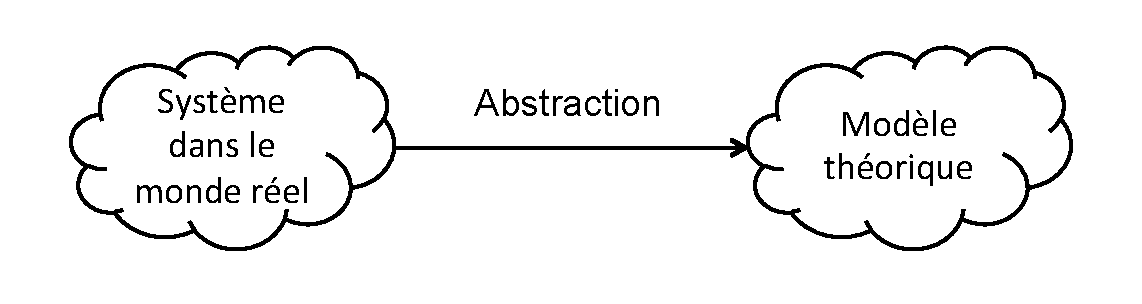
\includegraphics[scale=0.65]{images/Abstraction.pdf}
\end{center}

Afin de formaliser un système dans le monde réel, nous devons faire une abstraction vers un modèle théorique. Ce modèle théorique est un ensemble de phrases logiques dont il est possible de tirer des prédictions. Il n'est intéressant que s'il se comporte comme le vrai système.

Un exemple de cette formalisation pourrait être les équations de Maxwell qui sont le modèle théorique correspondant à la trajectoire des électrons et protons.

\subsection{Boucle de raisonnement}

Il existe trois formes de raisonnement: la déduction, l'induction et l'abduction. Ces trois formes de raisonnement peuvent être liées dans une boucle de raisonnement de la façon suivante:

\begin{center}
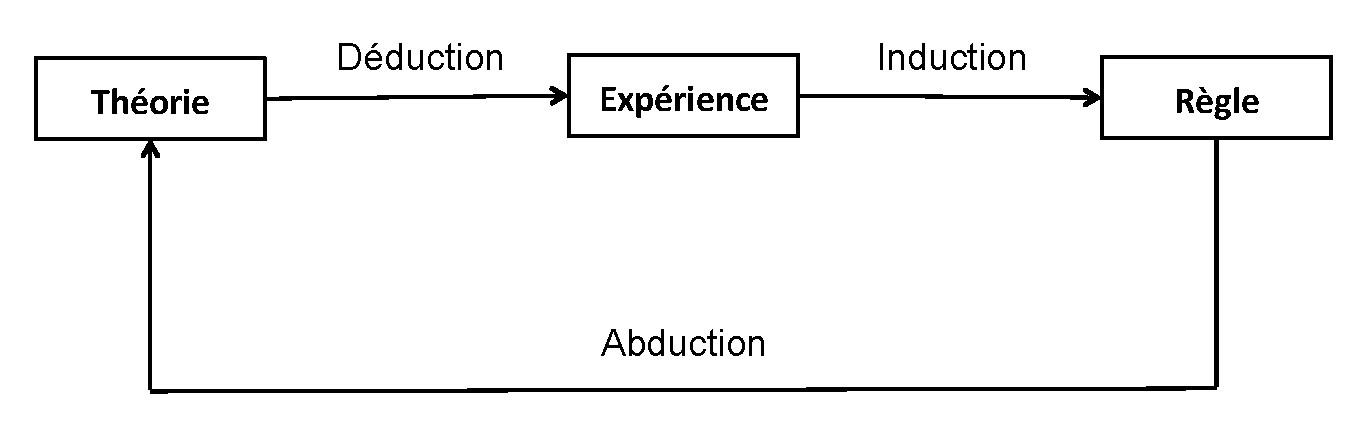
\includegraphics[scale=0.50]{images/BoucleRaisonnement1.pdf}
\end{center}

\subsubsection{Déduction}

Il s'agit de faire des calculs et des raisonnements logiques par rapport à la théorie. On en conclut une expérience. \\

\subsubsection{Induction}

L'induction est le fait de trouver une règle générale qui décrit les résultats d'expériences. On choisit en général une règle moyenne qui deviendra la règle générale.  Il faut souligner que les résultats expérimentaux ne sont pas totalement fiables ou incomplets. Dès lors, la règle trouvée n'est pas nécessairement exacte.  Par exemple, si par induction nous avons trouvé la règle, "les oiseaux volent", cela est vrai tant que l'on a pas vu un pingouin. Autre exemple, nous pouvons supposer que demain le soleil va se lever comme depuis des milliers d'années, même si rien ne l'assure.\\

\subsubsection{Abduction}

On compare la règle générale trouvée lors de l'induction avec la théorie. Si cela se révèle différent, comme l'on suppose que tout est parfait dans les calculs/expériences, c'est la théorie qui est fausse. Il faut alors corriger la théorie existante ou en inventer/deviner une nouvelle. Ce type de raisonnement est l'abduction. On applique l'abduction couramment dans notre vie de tous les jours; par exemple, lorsqu'un élève entre trempé dans la classe, nous supposons qu'il pleut dehors. \\


Sur ces trois concepts seul la déduction est un raisonnement sûr, les deux autres sont encore mal compris. Nous nous focaliserons dans ce cours uniquement sur la déduction. \\


\subsection{Exemples}

\subsubsection{Loi de Maxwell}

Nous illustrons dès à présent le fonctionnement de la boucle de raisonnement à l'aide de l'exemple cité plus haut, c'est-à-dire les équations de Maxwell :

\begin{center}
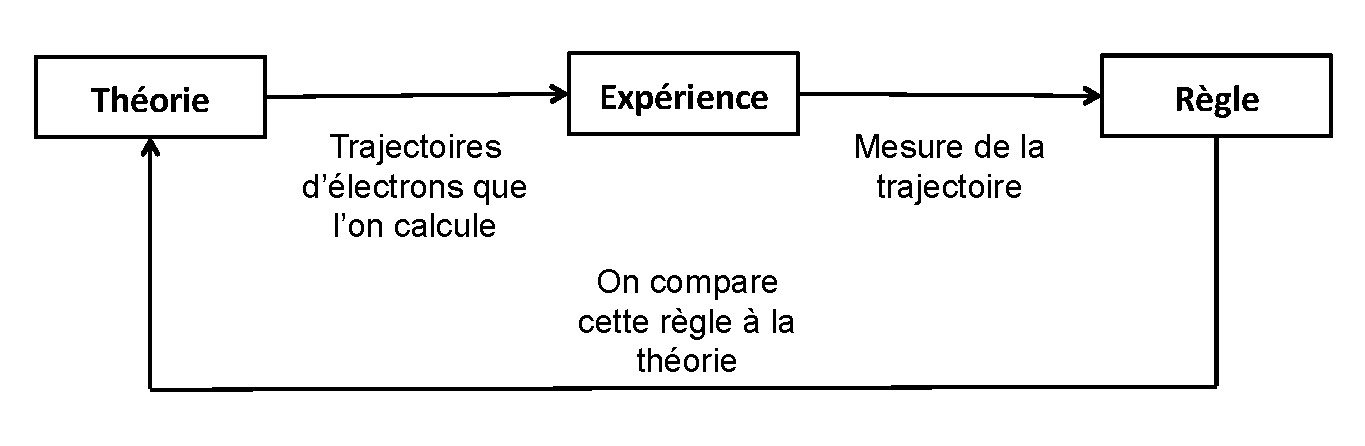
\includegraphics[scale=0.50]{images/BoucleRaisonnement2.pdf}
\end{center}

Par déduction, grâce à la théorie et aux conditions initiales que nous fixons, nous trouvons la trajectoire d'un électron. Nous effectuons ensuite des mesures dans le monde réel. Nous allons, par exemple, mesurer la trajectoire plusieurs fois avec des méthodes différentes et, par induction, nous trouvons une règle qui est la loi de comportement de la particule. Nous comparons ensuite, par abduction, cette règle à la théorie, et nous la corrigeons si besoin.\\



\subsubsection{Sac de billes}

Afin d'illustrer les 3 formes de raisonnement de manière plus formelle, considérons un sac de billes pouvant contenir des billes noires ou blanches. Notons que sac(x) signifie "la bille x est dans le sac" et que blanc(x) signifie "la bille x est blanche". \\

\paragraph{Déduction}

\begin{enumerate}
  \item Règle: $\forall$ $x$, $sac(x)$ $\Rightarrow$ $blanc(x)$
  \item Cas: $sac(a)$, $sac(b)$, $\cdots$\\
  \rule{5.5cm}{.1pt} 
  \item Résultat: $blanc(a)$, $blanc(b)$, $\cdots$
\end{enumerate}

Si toutes les billes se trouvant dans le sac sont blanches et que l'on pioche une bille de ce sac, cette bille sera blanche. Cette déduction est forcément correcte.

\paragraph{Induction}

\begin{enumerate}
  \item Cas: $sac(a)$, $sac(b)$,$\cdots$
  \item Résultat: $blanc(a)$, $blanc(b)$, $\cdots$\\
  \rule{5.5cm}{.1pt}	
  \item Règle: $\forall$ $x$, $sac(x)$ $\Rightarrow$ $blanc(x)$
\end{enumerate}

Si toutes les billes qu'on l'on pioche du sac sont blanches, alors nous pouvons établir comme règle que toutes les billes dans le sac sont blanches. Cette induction n'est pas forcément correcte.

\paragraph{Abduction}

\begin{enumerate}
  \item Règle: $\forall$ $x$, $sac(x)$ $\Rightarrow$ $blanc(x)$
  \item Résultat: $blanc(a)$, $blanc(b)$, $\cdots$\\
  \rule{5.5cm}{.1pt}
  \item Cas: $sac(a)$, $sac(b)$, $\cdots$
\end{enumerate}

Si toutes les billes se trouvant dans le sac sont blanches et que nous trouvons des billes blanches à côté du sac, nous pouvons penser qu'elles viennent du sac. Cette abduction n'est pas forcément correcte.

  \newpage
  
\chapter{La logique propositionnelle}

\begin{quote}
« \textit{\foreignlanguage{english}{They don't even need to know what they're
talking about.}} » --- Richard Feynman à propos des mathématiciens.
\end{quote}

La logique propositionnelle est la plus simple des formes de logique. Elle
permet de formaliser des expressions telles que les suivantes :

\begin{enumerate}
\item « S’il fait beau, alors je vais dehors. »
\item « Cet homme est grand et fort. »
\item « Il fait jour mais pas nuit. »
\end{enumerate}

Plus précisément, nous partons d’un ensemble de propositions
premières. Par exemple :

\begin{enumerate}
\item il fait beau ;
\item je vais dehors ;
\item cet homme est grand ;
\item cet homme est beau ;
\item il fait jour ;
\item il fait nuit.
\end{enumerate}

Le contenu exact de ces propositions n’a en fait aucune importance. C’est
pourquoi elles seront remplacées par des lettres majuscules :

\begin{enumerate}
\item A = « il fait beau » ;
\item B = « je vais dehors » ;
\item C = « cet homme est grand » ;
\item D = « cet homme est beau » ;
\item E = « il fait jour » ;
\item F = « il fait nuit ».
\end{enumerate}

Une proposition logique est alors :

\begin{itemize}
\item soit une des propositions premières ;
\item soit une combinaison de propositions logiques connectées par des
  connecteurs logiques.
\end{itemize}

Ainsi, les exemples de propositions précédentes peuvent être réécrits
comme ceci (la signification précise des différents symboles sera décrite
plus loin) :

\begin{enumerate}
\item $A \Rightarrow B$ ;
\item $C \land D$ ;
\item $E \land \lnot F$.
\end{enumerate}

% TODO: Plus d’exemples des différents connecteurs pour tout illustrer ? % On ne trouve pas nécessaire dans la mesure ou les trois exemple sont représentatifs - Cyril et Jon

L’avantage de cette notation par rapport aux phrases en français est qu’elle
nous permet d’effectuer des raisonnements formels sur les propositions
logiques. En particulier, nous pouvons précisément définir :

\begin{enumerate}
\item une \textbf{grammaire} qui définit ce qui est une proposition logique et ce qui
  ne l’est pas ;
\item une \textbf{sémantique} qui donne un sens à chaque proposition logique ;
\item une \textbf{théorie de preuve} permettant, en sachant qu’une proposition est
  vraie, de trouver d’autres propositions vraies (par exemple à partir de $A
  \Rightarrow B$ on peut trouver $\lnot B \Rightarrow \lnot A$).
\end{enumerate}
\section{La grammaire}

La logique propositionnelle est un \textbf{langage} formel. Il peut être défini
à l’aide d’une grammaire sur un \textbf{alphabet}. L’alphabet est l’ensemble des
symboles qui composent une proposition logique, c’est-à-dire :

\begin{itemize}
\item les lettres majuscules représentant les différentes propositions
  premières : $A$, $B$, $C$, etc. ;
\item $\true$ et $\false$ qui représentent des propositions qui sont
  respectivement toujours vraies et toujours fausses ;
\item les différents connecteurs logiques :
	\begin{itemize}
	\item Conjonction : $\land$
	\item Disjonction : $\lor$
	\item Négation :  $\lnot$
	\item Implication :  $\Rightarrow$
	\item Équivalence :  $\Leftrightarrow$
	\end{itemize}
\item les caractères de ponctuation « $($ » et « $)$ ».
\end{itemize}

Cependant, toutes les séquences composées de ces caractères ne sont pas des
phrases propositionnelles. La grammaire suivante permet de donner les règles que
les phrases propositionnelles doivent respecter~:

\begin{tabular}{rl}
  $\textrm{<identificateur>}$ & = $A$ | $B$ | $C$ | $D$ | \dots \\
  $\textrm{<proposition>}$
  & = $\true$ \\
  & | $\false$ \\
  & | $\textrm{<identificateur>}$ \\
  & | $(\textrm{<proposition>})$ \\
  & | $\lnot \textrm{<proposition>}$ \\
  & | $\textrm{<proposition>} \land \textrm{<proposition>}$ \\
  & | $\textrm{<proposition>} \lor \textrm{<proposition>}$ \\
  & | $\textrm{<proposition>} \Rightarrow \textrm{<proposition>}$ \\
  & | $\textrm{<proposition>} \Leftrightarrow \textrm{<proposition>}$
\end{tabular}
\vspace{2 mm}

Remarquez que seules les séquences de symboles qui respectent cette
grammaire sont des phrases propositionnelles. Ainsi, $p \Leftrightarrow q$
n’est pas une phrase propositionnelle parce que les propositions
premières sont des lettres majuscules ; de même les phrases en français —
ou en klingon, ou encore dans d’autres formalismes mathématiques – comme «
  s’il fait beau alors je vais dehors » ne respectent pas la grammaire
précédente et ne sont donc pas des phrases propositionnelles.

Notez aussi que le discours à propos des phrases propositionnelles n’est
pas une phrase propositionnelle. La grammaire précédente, la description de
l’alphabet, et cette explication parlent de propositions logiques sans en
être, et font donc partie de ce qui est appelé le \textbf{métalangage}.

\section{Les tables de vérité}

La grammaire permet de définir précisément l’ensemble des phrases
propositionnelles, mais pas de leur donner un sens, c’est-à-dire de définir
quand une proposition est vraie ou fausse.

Pour cela, il faut décider lesquelles des propositions premières sont vraies
et lesquelles sont fausses. Rappelez-vous que la signification des
propositions premières n’a aucune importance, ce choix est donc complètement
arbitraire (le choix qui décrit au mieux le monde réel n’est qu’un des choix
possibles parmi tous les autres). On sait également que les propositions
$\true$ et $\false$ sont, respectivement, toujours vraies et toujours
fausses.

Les autres propositions sont construites à partir de propositions plus
simples. Leur véracité est fonction de celle des propositions qui les
composent. Prenons par exemple $p \land q$, où $p$ et $q$ sont d’autres
propositions. La véracité de $p \land q$ est une fonction de celle de $p$ et
de $q$ : $p \land q$ est vrai si et seulement si $p$ et $q$ sont vrais aussi
($\land$ est un « et » logique). Cette relation peut être exprimée à l’aide
de la table de vérité suivante :

\vspace{2 mm}
\begin{tabular}{ll|l}
  $p$ & $q$ & $p \land q$ \\
  \hline

  $\true$ & $\true$ & $\true$ \\
  $\true$ & $\false$ & $\false$ \\
  $\false$ & $\true$ & $\false$ \\
  $\false$ & $\false$ & $\false$
\end{tabular}

\vspace{2 mm}
Voici la table de vérité des autres connecteurs logiques :
\vspace{2 mm}

\begin{tabular}{ll|l}
  $p$ & $q$ & $p \lor q$ \\
  \hline

  $\true$ & $\true$ & $\true$ \\
  $\true$ & $\false$ & $\true$ \\
  $\false$ & $\true$ & $\true$ \\
  $\false$ & $\false$ & $\false$
\end{tabular}
\vspace{2 mm}

\begin{tabular}{ll|l}
  $p$ & $q$ & $p \Leftrightarrow q$ \\
  \hline

  $\true$ & $\true$ & $\true$ \\
  $\true$ & $\false$ & $\false$ \\
  $\false$ & $\true$ & $\false$ \\
  $\false$ & $\false$ & $\true$
\end{tabular}
\vspace{2 mm}

\begin{tabular}{l|l}
  $p$ & $\lnot p$ \\
  \hline

  $\true$ & $\false$ \\
  $\false$ & $\true$
\end{tabular}
\vspace{2 mm}

\begin{tabular}{ll|l}
  $p$ & $q$ & $p \Rightarrow q$ \\
  \hline

  $\true$ & $\true$ & $\true$ \\
  $\true$ & $\false$ & $\false$ \\
  $\false$ & $\true$ & $\true$ \\
  $\false$ & $\false$ & $\true$
\end{tabular}
\vspace{2 mm}

Remarquez que le dernier tableau est correct. Il n’est parfois pas intuitif
que la proposition $A \Rightarrow B$ (qui pourrait s’exprimer en français
par « si $A$, alors $B$ ») soit toujours vraie quand $A$ est faux, mais c’est
pourtant le cas : la proposition dit que quand $A$ est vrai, $B$ doit
l’être aussi, mais elle ne donne aucune information sur le cas où $A$ est
faux.

Les parenthèses, quant à elles, servent à distinguer des propositions telles
que $A \land (B \lor C)$ et $(A \land B) \lor C$, qui s’écriraient de la
même manière sans parenthèses alors qu’elles n’ont pas la même table de
vérité :

\begin{tabular}{lll|ll}
  $A$ & $B$ & $C$ & $A \land (B \lor C)$ & $(A \land B) \lor C$ \\
  \hline

  $\true$  & $\true$  & $\true$  & $\true$  & $\true$  \\
  $\true$  & $\true$  & $\false$ & $\true$  & $\true$  \\
  $\true$  & $\false$ & $\true$  & $\true$  & $\true$  \\
  $\true$  & $\false$ & $\false$ & $\false$ & $\false$ \\
  $\false$ & $\true$  & $\true$  & $\false$ & $\true$  \\
  $\false$ & $\true$  & $\false$ & $\false$ & $\false$ \\
  $\false$ & $\false$ & $\true$  & $\false$ & $\true$  \\
  $\false$ & $\false$ & $\false$ & $\false$ & $\false$
\end{tabular}

\section{Les interprétations}

Une autre façon plus puissante de définir si une proposition est vraie ou fausse est d’utiliser
une \textbf{interprétation}. Si $E_P$ est l’ensemble des propositions premières,
alors une interprétation $I$ définit la fonction $\val_I : E_P \rightarrow
\{\true, \false\}$ \footnote{La notation $f : A \rightarrow B$ signifie que $f$
  est une fonction depuis l’ensemble $A$ vers l’ensemble $B$.  } qui permet de
savoir si ces propositions premières sont vraies ou fausses. Par exemple, on
pourrait écrire ceci :

\[\val_I(A) = \true\]
\[\val_I(B) = \false\]
\[\val_I(C) = \true\]

Étant donné la fonction $\val_I$, il est possible de définir la fonction
$\VAL_I : P \rightarrow \{\true, \false\}$, qui est une extension de
$\val_I$ à $P$, l’ensemble de toutes les propositions. L’équivalent des
tables de vérité pourrait être des expressions telles que~:

\[\forall p \in E_P. \VAL_I(p) = \val_I(p)\]

% Les définitions du type « A \land B est vrai si A et B sont vrais » me
% paraissent être cycliques, donc je les ai plutôt écrites comme ça, mais je ne
% sais pas si cela paraît évident pour tout le monde.
\[\VAL_I(p \land q) = \begin{cases}
  \true \mbox{ si } \VAL_I(p) \mbox{ et } \VAL_I(q) = \true \\
  \false\mbox{ sinon}
\end{cases}\]

\[\VAL_I(p \lor q) = \begin{cases}
  \false \mbox{ si } \VAL_I(p) \mbox{ ou } \VAL_I(q) = \false \\
  \true\mbox{ sinon}
\end{cases}\]

\[\VAL_I(\lnot p) = \begin{cases}
  \false\mbox{ si }\VAL_I(p) = \true \\
  \true\mbox{ si }\VAL_I(p) = \false
\end{cases}\]

\[\VAL_I(p \Leftrightarrow q) = \begin{cases}
  \true\mbox{ si }\VAL_I(p) = \VAL_I(q) \\
  \false\mbox{ sinon}
\end{cases}\]

\[\VAL_I(p \Rightarrow q) = \begin{cases}
  \false \mbox{ si } \VAL_I(q) = \false \mbox{ alors que } \VAL_I(p) = \true \\
  \true\mbox{ sinon}
\end{cases}\]

Prenons un exemple concret, utilisons une interprétation pour étudier la phrase
suivante~: « S'il fait beau à midi, j'irai promener le chien ». Nous devons
d’abord traduire cette phrase en l’une des propositions du formalisme que nous
avons défini, en commençant par identifier les propositions premières~:

\begin{enumerate}
\item B = « Il fait beau »~;
\item M = « Il est midi »~;
\item P = « Je vais promener le chien »~;
\end{enumerate}

Identifions également les connecteurs à employer~: « s’il fait beau $\land$
  qu'il est midi $\Rightarrow$ j’irai promener le chien ». En combinant ces deux
résultats, nous obtenons la phrase propositionnelle $(B \land M) \Rightarrow P$.

Interprétons désormais notre proposition à l’aide de l’interprétation suivante~:
\begin{enumerate}
  \item Il fait beau~: $\val_I(B) = \true$~;
  \item Il est midi~: $\val_I(M) = \true$~;
  \item Je n’irai pas promener le chien~: $\val_I(P) = \false$.
\end{enumerate}

Nous pouvons alors effectuer le développement suivant~:

\begin{align*}
  \VAL_I((B \land M) \Rightarrow P) &= \begin{cases}
    \false \mbox{ si } \VAL_I(P) = \false \mbox{ alors que } \VAL_I(B \land M) = \true \\
    \true\mbox{ sinon}
  \end{cases} \\
  \mbox{ or }\VAL_I(B \land M) &= \begin{cases}
    \true \mbox{ si } \VAL_I(B) \mbox{ et } \VAL_I(M) = \true \\
    \false\mbox{ sinon}
  \end{cases} \\
  &= \true \\
  \mbox{ donc }  \VAL_I((B \land M) \Rightarrow P) &= \begin{cases}
    \false \mbox{ si } \VAL_I(P) = \false \\
    \true\mbox{ sinon}
  \end{cases} \\
  &= \false
\end{align*}

Nous pouvons donc conclure que, dans cette interprétation, la personne ayant
fait cette affirmation a menti. Notons néanmoins que notre homme n'aurait pas
menti en partant promener le chien alors qu'il pleuvait à midi, rien n'ayant
été dit sur ce qu'il ferait dans le cas où il ne ferait pas beau.

% TODO: Rajouter un exemple simple pour vérifier que l’un des connecteurs est
% bien défini (\land, etc.) et aussi montrer la démarche :
%   - avoir une phrase en français avec 2-3 connecteurs logiques ;
%   - identifier les propositions primaires et les connecteurs ;
%   - réécrire la phrase mathématiquement ;
%   - définir une interprétation ;
%   - l’utiliser pour évaluer la fonction.

\section{Les modèles logiques}

À partir de la notion d’interprétation, nous pouvons définir ce qu’est
un \textbf{modèle}. Soit $B = \{b_1, b_2, \dots, b_n \}$ un ensemble de
propositions logiques. Une interprétation $I$ est un modèle de $B$ si et
seulement si $\forall b_i \in B. \VAL_I(b_i) = \true$. Autrement dit, $I$
décris un univers qui respecte toutes les règles se trouvant dans l’ensemble
$B$.

Donc, dans notre exemple précédent, l’interprétation choisie n’est pas un modèle
de la proposition analysée, celle-ci n’étant pas validée, mais par exemple
l’interprétation telle que $\val_I(B) = \true$, $\val_I(M) = \true$ et
$\val_I(P) = \true$ est bien un modèle de la proposition utilisée comme
exemple. Remarquez aussi que cela ne change rien au fait que l’interprétation
choisie est le modèle d’autres propositions que celle étudiée (par exemple $B
\land M$).

% TODO: Exemple d’expression avec une interprétation qui est un modèle et une
% autre qui n’en est pas un.
\begin{description}\item[Les tautologies :] Pour certaines propositions, toute interprétation est un modèle, c’est-à-dire que ces propositions sont toujours
  vraies. Par exemple, $\true$ est évidemment une tautologie, de même que $A
  \Rightarrow A$ ou encore $A \lor \lnot A$. Le fait qu’une proposition $p$ est
  une tautologie se note $\vDash p$.
\item[Les contradictions :] Pour d’autres propositions, il n’existe aucun
  modèle, c’est-à-dire qu’elles sont toujours fausses. Par exemple $A \land
  \lnot A$ est une contradiction. Le fait qu’une proposition $p$ est une
  contradiction se note $\nvDash p$.
\item[Les contingences :] Toutes les autres propositions sont des contingences. Il
  existe des interprétations qui sont des modèles et d’autres qui n’en sont
  pas. Par exemple $A \land B$ est vrai pour l’interprétation $I$ telle que
  $\val_I(A) = \val_I(B) = \true$, mais faux dans tous les autres cas.
\end{description}

		\subsection{Conséquence logique}
			$p$ est conséquence logique de $q$ si et seulement si $p \Rightarrow q$ est une tautologie. En d'autres termes, si
			\begin{center}
			\begin{tabular}{ll}
			$p \models q$ & $q$ est valide dans tous les modèles de $p$ \\
			&\\
			alors & \\
			$\models (p \Rightarrow q)$ & $p \Rightarrow q$ est une tautologie.\\
			&\\
			On peut donc écrire & \\
			$p \Rrightarrow q$ & $p$ est conséquence logique de $q$.\\
			\end{tabular}
			\end{center}
			Cependant, la conséquence logique ($\Rrightarrow$) n'est pas une proposition logique (cf. syntaxe d'une proposition).
		
		\subsection{Équivalence logique}
			Par le raisonnement ci-dessus, on peut dire que $p$ est logiquement équivalent à $q$ si et seulement si
			\begin{center}
			\begin{tabular}{ll}
			$p \models q$ & $q$ est valide dans tous les modèles de $p$ \\
			$q \models p$ & $p$ est valide dans tous les modèles de $q$ \\
			&\\
			et donc & \\
			$\models (p \Rightarrow q)$ & $p \Rightarrow q$ est une tautologie et\\
			$\models (q \Rightarrow p)$ & $q \Rightarrow p$ est une tautologie.\\
			&\\
			On peut donc écrire & \\
			%impossible de trouver l'équivalence logique en symbole
			$p \Lleftarrow \Rrightarrow q$ & $p$ sont logiquement équivalents $q$.\\ 
			\end{tabular}
			\end{center}
			L'équivalence logique n'est pas non plus une proposition logique.\\
			
			Il ne faut pas non plus oublier la différence entre phrase propositionnelle ($p$, $q$, $s$,...) et propositions primaires ($P$, $Q$, $S$,...) (cf. syntaxe d'une proposition) :
			\begin{center}
			\begin{tabular}{ll}
				$p \Rightarrow q$ & n'est pas une proposition\\
				
				mais &\\
				$P \land Q \Rightarrow R \land \lnot S$ & en est bien une.\\
			\end{tabular}
			\end{center}
	

  \newpage
  % \documentclass[10pt,a4paper]{article}
% \usepackage[utf8]{inputenc}
% \usepackage{amsmath}
% \usepackage{amsfonts}
% \usepackage{amssymb}
% \usepackage{array}
% \begin{document}
%% 	\chapter{Rappel}
% 		\subsection{Conséquence logique}
% 			$p$ est conséquence logique de $q$ si et seulement si $p \Rightarrow q$ est une tautologie. En d'autres termes, si
% 			\begin{center}
% 			\begin{tabular}{ll}
% 			$p \models q$ & $q$ est valide dans tous les modèles de $p$ \\
% 			&\\
% 			alors & \\
% 			$\models (p \Rightarrow q)$ & $p \Rightarrow q$ est une tautologie.\\
% 			&\\
% 			On peut donc écrire & \\
% 			$p \Rrightarrow q$ & $p$ est conséquence logique de $q$.\\
% 			\end{tabular}
% 			\end{center}
% 			Cependant, la conséquence logique ($\Rrightarrow$) n'est pas une proposition logique (cf. syntaxe d'une proposition).
% 		
% 		\subsection{Équivalence logique}
% 			Par le raisonnement ci-dessus, on peut dire que $p$ est logiquement équivalent à $q$ si et seulement si
% 			\begin{center}
% 			\begin{tabular}{ll}
% 			$p \models q$ & $q$ est valide dans tous les modèles de $p$ \\
% 			$q \models p$ & $p$ est valide dans tous les modèles de $q$ \\
% 			&\\
% 			et donc & \\
% 			$\models (p \Rightarrow q)$ & $p \Rightarrow q$ est une tautologie et\\
% 			$\models (p \Rightarrow q)$ & $p \Rightarrow q$ est une tautologie.\\
% 			&\\
% 			On peut donc écrire & \\
% 			%impossible de trouver l'équivalence logique en symbole
% 			$p \Lleftarrow \Rrightarrow q$ & $p$ est conséquence logique de $q$.\\ 
% 			\end{tabular}
% 			\end{center}
% 			L'équivalence logique n'est pas non plus une proposition logique.\\
% 			
% 			Il ne faut pas non plus oublier la différence entre phrase propositionnelle ($p$, $q$, $s$,...) et propositions primaires ($P$, $Q$, $S$,...) (cf. syntaxe d'une proposition) :
% 			\begin{center}
% 			\begin{tabular}{ll}
% 				$p \Rightarrow q$ & n'est pas une proposition\\
% 				
% 				mais &\\
% 				$P \land Q \Rightarrow R \land \lnot S$ & en est bien une.\\
% 			\end{tabular}
% 			\end{center}
% 	
	\chapter{Les preuves}
		Une preuve est une manière de partir d’une formule et de dire si celle-ci est vraie ou fausse.\\
		il y a 3 approches possibles :
		\begin{itemize}
			\item Table de vérité
			\item Preuve transformationnelle
			\item Preuve déductive (la plus générale)		
		\end{itemize}
		\section{Preuve avec table de vérité}
			\newcolumntype{x}{>{\itshape\bfseries}c}
		Prouvons que $\lnot (P \land Q) \Leftrightarrow (\lnot P \lor \lnot Q)$ est vrai :
			\begin{center}
			\begin{tabular}{cc|ccxcx}
			$P$ & $Q$ & $\lnot P$ & $\lnot Q$ & $(\lnot P \lor \lnot Q)$ & $P \land Q$ & $ (\lnot P \lor \lnot Q)$\\
			\hline
			F&F&T&T&T&F&T\\
			T&F&F&T&T&F&T\\
			F&T&T&F&T&F&T\\
			T&T&F&F&F&T&F\\
			\end{tabular}
			\end{center}
			On voit bien ici, que la table de $\lnot (P \land Q)$ est équivalente à celle de $\lnot (P \land Q)$. La preuve a donc vérifié la véracité de la proposition. \\
			Il y a néanmoins un problème avec cette preuve, car s'il y a $N$ propositions premières, on a $2^N$ lignes dans la table.
		\section{Preuve transformationnelle}
			On va utiliser des "Lois", c'est-à-dire des équivalences.
			\begin{center}
			\begin{tabular}{|ll|}
			\hline
			$p \Lleftarrow \Rrightarrow p \lor p$ & Idempotence\\
			$p \lor q \Lleftarrow \Rrightarrow q \lor p$ & Commutativité\\
			$(p \lor q) \lor r \Lleftarrow \Rrightarrow p \lor (q \lor r)$ & Associativité\\
			$ \lnot \lnot p \Lleftarrow \Rrightarrow p$ & Double Négation\\
			$p \Rightarrow q \Lleftarrow \Rrightarrow \lnot p \lor q$ & Implication\\
			$\lnot (p \land q) \Lleftarrow \Rrightarrow \lnot p \lor \lnot q$ & $1^{ere}$ loi de De Morgan\\
			$p \Leftrightarrow q \Lleftarrow \Rrightarrow (p \Rightarrow q) \land (q \Rightarrow p)$ & Équivalence\\
			\hline
			\end{tabular}
			\end{center}
			On y ajoute 2 règles supplémentaires pour cette technique : 
			\subsection*{Transitivité de l'équivalence}
			\indent Si $p \Lleftarrow \Rrightarrow q$ et $q \Lleftarrow \Rrightarrow r$, alors $p \Lleftarrow \Rrightarrow r$.
			\subsection*{Substitution}
			Il est autorisé de remplacer une formule par une formule équivalente à l’intérieur d’une autre formule. Autrement dit : \\
			\indent Soit p,q,r des formules propositionnelles.\\
			\indent Si $p \Leftrightarrow q$ et $r(p)$, alors $r(p) \Lleftarrow \Rrightarrow r(q)$.\\
			On peut remplacer $p$ par $,q$ car elles sont équivalentes. Il faut faire attention à ces règles, car elles sont en métalangage. Elles expliquent seulement ce qui est autorisé  faire.
			
			\subsection*{Exemple}
			On veut prouver : $p \land (q \land r) \Lleftarrow \Rrightarrow (p \land q) \land r$
			\begin{center}
			\begin{tabular}{ll}
			
			$p \land (q \land r)$ & $\Lleftarrow \Rrightarrow p \land \lnot \lnot (q \land r)$\\
			& $\Lleftarrow \Rrightarrow p \land \lnot (\lnot q \lor \lnot r)$\\
			& $\Lleftarrow \Rrightarrow \lnot \lnot (p \land \lnot (\lnot q \lor \lnot r))$\\
			& $\Lleftarrow \Rrightarrow \lnot (\lnot p \lor \lnot \lnot (\lnot q \lor \lnot r))$\\
			& $\Lleftarrow \Rrightarrow \lnot (\lnot p \lor (\lnot q \lor \lnot r))$\\
			& $\Lleftarrow \Rrightarrow \lnot ((\lnot p \lor \lnot q) \lor \lnot r)$\\
			&$\vdots$\\
			& effectuer les mêmes lois dans le sens contraire \\
			&$\vdots$\\
			& $\Lleftarrow \Rrightarrow (p \land q) \land r$\\
			\end{tabular}
			\end{center}
			Le problème dans cette méthode de preuve c'est qu'il faut de l'idée, de la créativité et donc ce n'est pas forcément mieux que les tables de vérité, surtout si c'est compliqué de trouver l'astuce.
		
		\section{Preuve déductive}
		À partir des lois logiques (lois d'équivalence) et des règles d'inférence, on va construire des preuves.\\
		\textit{Une preuve est un objet formel défini avec précision.\\}
		
		Equivalences logiques : 	
			\begin{center}
			\begin{tabular}{ll}
			$p \Lleftarrow \Rrightarrow p \lor p$ & Idempotence de $\lor$\\
			$p \lor q \Lleftarrow \Rrightarrow q \lor p$ & Commutativité de $\lor$\\
			$(p \lor q) \lor r \Lleftarrow \Rrightarrow p \lor (q \lor r)$ & Associativité de $\lor$\\
			$ \lnot \lnot p \Lleftarrow \Rrightarrow p$ & Double Négation\\
			$p \Rightarrow q \Lleftarrow \Rrightarrow \lnot p \lor q$ & Implication\\
			$\lnot (p \land q) \Lleftarrow \Rrightarrow \lnot p \lor \lnot q$ & $1^{ere}$ loi de De Morgan\\
			$\lnot (p \lor q) \Lleftarrow \Rrightarrow \lnot p \land \lnot q$ & $2^{eme}$ loi de De Morgan\\
			$(p \land q) \lor r \Lleftarrow \Rrightarrow (p \lor r) \land (q \lor r)$ & Distributivité de $\lor$\\
			\end{tabular}
			\end{center}
			Mais également l'idempotence, la commutativité, l'associativité et la distributivité de $\land$.\\
			
		Règle d'inférence : \\
		
		À la différence de la preuve transformationnelle, les règles d'inférences ont une direction : elles commencent par les prémisses et se terminent par la conclusion.
		\begin{center}
		\begin{tabular}{llp{3cm}l}
		
   			Conjonction : &
   			\begin{tabular}{cl}
      		p & prémisse\\
      		q & prémisse\\
      		\line(1,0){25}&\\
      		$p\land q$ & Conclusion
   			\end{tabular} 
   			&
   			
   			Simplification : &
   			\begin{tabular}{c}
      		$p \land q$ \\
      		\hline
      		$p$\\
   			\end{tabular} \\
   			&\\
   			
   			Addition : &
   			\begin{tabular}{c}
      		$p $ \\
      		\hline
      		$p \lor q$\\
   			\end{tabular}
   			&
   			
   			Contradiction : &
   			\begin{tabular}{c}
      		$p$ \\
      		$\lnot p$\\
      		\hline
      		$q$\\
   			\end{tabular}\\
   			&\\
   			
   			Double Négation : &
   			\begin{tabular}{c}
      		$\lnot \lnot p $ \\
      		\hline
      		$p$\\
   			\end{tabular}
   			&
   			
   			\raggedright Transitivité de l'équivalence : &
   			\begin{tabular}{c}
      		$p \Leftrightarrow q$ \\
      		$q \Leftrightarrow r$ \\
      		\hline
      		$p \Leftrightarrow r$\\
   			\end{tabular}\\
   			&\\
   			
   			Modus Ponens : &
   			\begin{tabular}{c}
      		$p \Rightarrow q$ \\
      		$p$ \\
      		\hline
      		$q$\\
   			\end{tabular}
   			&
   			
   			Modus Tollens : &
   			\begin{tabular}{c}
      		$p \Rightarrow q$ \\
      		$\lnot q$ \\
      		\hline
      		$\lnot p$\\
   			\end{tabular}\\
   			&\\
   			
   			Loi d'équivalence : &
   			\begin{tabular}{c}
      		$p \Leftrightarrow q$ \\
      		\hline
      		$q \Leftrightarrow p$\\
   			\end{tabular}\\		
		\end{tabular}
		\end{center}
		
		On y ajoute 2 règles spéciales : 
		\begin{itemize}
		\item Le théorème de déduction,
		\item La preuve par contradiction.
		\end{itemize}
		
		\subsection*{Théorème de déduction}
			Pour prouver $s\Rightarrow t$, on suppose $s$ vrai. On déduit $t$ et donc on sait que l'hypothèse $s\Rightarrow t$ est vraie et on l'évacue.\\
			
			On note ce théorème $s \vdash t$ (t peut être prouvé à partir de s, ce qui signifie qu'on peut construire une preuve (objet mathématique) qui est vraie si on applique bien les règles ci-dessus).\\
			
			\textbf{Remarque :} $p\models t \neq p\vdash t$
			\begin{itemize}
			\item $p\models t$ est une notion de vérité, et donc de sémantique;
			\item $ p\vdash t$ est une notion syntaxique, on peut prouver qu'une preuve est vraie.
			\end{itemize}
			
			Notion de prouvabilité : on peut créer une preuve, et donc on peut créer une séquence de prémisses et de conclusions.
			\begin{center}
			\begin{tabular}{c}
      		$p,...,r,s \vdash t$ \\
      		\hline
      		$p,...,r \vdash s\Rightarrow t$\\
   			\end{tabular}\\
			\end{center}
			Ceci permet notamment de formaliser des théorèmes.
			
		\subsection*{Preuve par contradiction}
		C'est une preuve indirecte :\\
		Implicitement, on suppose que $p$ jusqu'à $q$ n'a pas de problème, c'est-à-dire qu'on ne peut pas prouver une contradiction pour ces formules propositionnelles.
		\begin{center}
			\begin{tabular}{c}
      		$p,...,q,r \vdash s$ \\
      		$p,...,q,r \vdash \lnot s$\\
      		\hline
      		$p,...,q \vdash \lnot r$\\
   			\end{tabular}\\
			\end{center}
			
			Ceci signifie qu'il y a une erreur dans les prémisses, et on suppose ici que c'est la formule propositionnelle $r$ qui est fautive. On justifie qu'il n'y a aucune contradiction dans $,p,...,q$ car on part du principe qu'il existe un modèle de $p,...q$.\\
			
			Tout ceci est une formalisation de choses qu'on connaît déjà, mais ça nous donne une notion précise du raisonnement à avoir.
			
\section{Exemple de preuve propositionnelle}

\noindent Voici les propositions premières : \\
A : tu manges bien \\
B : ton système digestif est en bonne santé \\
C : tu pratiques une activité physique régulière \\
D : tu es en bonne forme physique \\
E : tu vis longtemps \\

\noindent On peut maintenant faire une théorie et on espère qu'elle aura un modèle. \\
A$\Rightarrow$B, C$\Rightarrow$D, B$\lor$D $\Rightarrow$ E, $\lnot$E
\\
\noindent On aimerait prouver que $\lnot$A $\land$ $\lnot$C est vrai.\\

\noindent Preuve : \\
\\
\begin{tabular}{|l|l|}
\hline
1. A$\Rightarrow$B & prémisse \\
2. C$\Rightarrow$D & prémisse \\
3. B$\lor$D $\Rightarrow$E & prémisse \\
4. $\lnot$E & prémisse \\ 
\indent 5. A & hypothèse \\
\indent 6. B & modus ponens (1) \\
\indent 7. B$\lor$D & addition (6) \\
\indent 8. E & modus ponens (7) \\
9. $\lnot$A & preuve indirecte \\
\indent 10. C & hypothèse \\
\indent 11. D & modus ponens (2) \\
\indent 12. D$\lor$B & addition (11) \\
\indent 13. B$\lor$D & commutativité (12)\\
\indent 14. E & modus ponens (9) \\
15. $\lnot$C & preuve indirecte \\
16. $\lnot$A $\land$ $\lnot$C & conjonction (9,15) \\
\hline
\end{tabular}\\

Grâce à la déduction, on a donc pu prouver que tu ne manges pas bien et que tu ne pratiques pas d'activité physique régulière. 
On aimerait maintenant pouvoir automatiser les preuves quand elles existent. Mais il faut savoir s'il peut tout résoudre ou pas. 
On va donc construire un algorithme nous permettant de résoudre automatiquement les preuves en logique propositionnelle.

% \end{document}

  \newpage
  
\chapter{Deux règles plus sophistiquées}

\section{Théorème de déduction}

\begin{itemize}
\item  Pour prouver s $\Rightarrow$ t
\item  On suppose s vrai
\item  On déduit t
\item  Ensuite on évacue l'hypothèse
\end{itemize}


\textit{Notation: p $\vdash$ t (on peut prouver t à partir de p) }

\subsection{Prémisse:}

\begin{equation}
\frac{p........................r, s \vdash t} 
{p........................r, s \vdash (s \Rightarrow t)}
\end{equation}

\subsection{Conclusion:}

Déduire une implication

\section{Preuve par contradition (ou preuve indirecte)}

On prend un hypothèse, et on peut prouver qu'elle est vraie ou fausse, d'où l'hypothèse n'est pas bonne.

\subsection{Prémisse:} 
on suppose que p...q n'a pas de problème

\begin{equation}
\begin{split}
p........................q, r, s \vdash s \\
\frac{p........................ q,r, s \vdash \lnot s}
{p........................ q \vdash \lnot r}
\end{split}
\end{equation}

\subsection{Conclusion:}

si p...q n'a pas de problème, on se focalise alors sur r
 

\chapter{Exemples de Preuves}

Une preuve est une séquence de pas où chaque pas est une application de règles d'inférences et de lois logiques
Il faut justifier à chaque étape le nom de la règle / loi, et indenter les éléments de la preuve en preuve conditionnelle indirecte.

\section{Prémisse:} 

p $\land$ q $\lor$ r

\section{Conclusion:}

$\lnot$ p $\Rightarrow$ r

\section{Exemple sans preuve conditionnelle}

\begin{enumerate}
\item   (p $\land$ q) $\lor$ r  \textit{Prémisse}
\item   r $\lor$ (p $\land$ q)  $\lor$ r \textit{Commutativité en 1}
\item   (r $\lor$ p) $\land$ (r$\lor$q) \textit{Associativité en 2}
\item   (r $\lor$ p) \textit{Simplification en 3}
\item   (p $\lor$ r) \textit{Commutativité en 4}
\item   $\lnot$$\lnot$ p $\lor$ r \textit{Loi de la négation en 5}
\item   $\lnot$ p $\Rightarrow$ r \textit{Implication en 6}
\end{enumerate}

\section{Exemple avec preuve conditionnelle}

\begin{enumerate}
\item (p $\land$ q) $\lor$ r  \textit{Prémisse}
\item $\lnot$ $\lnot$(p $\land$ q) $\lor$ r \textit{Double négation en 1}
\item $\lnot$ ( $\lnot$ p $\land$ $\lnot$ q) \textit{Loi De Morgan en 2}
\item $\lnot$ p $\lor$ $\lnot$ q $\Rightarrow$ r \textit{Implication en 3}

\begin{enumerate}
 \item  $\lnot$ p \textit{Hypothèse}
 \item  $\lnot$ p $\lor$ $\lnot$ p \textit{ Addition sur 5}
 \item  r \textit{ Modus Ponens sur 4 et 6}
\end{enumerate}

\item  $\lnot$ p $\Rightarrow$ r \textit{Evacuation de l'hypothèse}
\end{enumerate}

\section{Exemple de Preuve par contradiction}

\begin{enumerate}
\item  (p $\land$ q) $\lor$ r  \textit{Prémisse}
\item  (p  $\lor$ r) $\land$ (q $\lor$ r) \textit{Distributivité sur 1}
\item  (p $\lor$ r)  \textit{Simplification en 2}

\begin{enumerate}
 \item $\lnot$ ( $\lnot$ p $\Rightarrow$ r)  \textit{Hypothèse}
 \item $\lnot$ ( $\lnot$ $\lnot$ p $\lor$ r)\textit{Implication en 4}
 \item $\lnot$ (p $\lor$ r) \textit{ Négation en 5}
\end{enumerate}

\item $\lnot$ $\lnot$ ($\lnot$ p $\Rightarrow$ r)  \textit{ Preuve par contradiction}
\item $\lnot$ p $\Rightarrow$ r \textit{Négation en 7}
\end{enumerate}


\chapter{Quelques concepts}
\section{Principe de dualité }

\subsection{Dans les formules sans $\rightarrow$ :}

\begin{equation}
1 \leftrightarrow T \hspace{5cm} true \leftrightarrow false 
\end{equation}
\begin{align*}
\models \lnot ( p \land q)  \Leftrightarrow \lnot p \lor \lnot q \\
\models \lnot ( p \lor q)  \Leftrightarrow \lnot p \land \lnot q 
\end{align*}

\subsection{Formule quelconque:}

\begin{equation}
	1 \leftrightarrow T \hspace{5cm} true \leftrightarrow false 
\end{equation}

 Justification en raisonnant sur les modèles:
 \begin{align*}
	 p1,...,pn \models ssi \models (p1,...,pn \land \lnot q) \leftrightarrow false \\
	 ssi \models ( \lnot p1 \lor ... \lor pn) \leftrightarrow true
 \end{align*}

\section{Forme Normale}

\begin{itemize}
  \item Conjonctive: $( p \lor q ) \land ( q \lor a ) \land ( s \lor r )$  
  \item Disjonctive
\end{itemize}

\subsection{terminologie}

\begin{itemize}
	\item Littéral :$ P \lor \lnot P \approxeq L$
	\item Clause : $\lor L{i} = ( L{1} \lor L{2} \lor L{3} ... \lor L{i} )$
\end{itemize}

\subsection{Forme normale conjonctive FNC}

\section{Algorithme de normalisation}

\begin{enumerate}
\item Eliminer les $\rightarrow$ et $\leftrightarrow$
\item Déplacer les négations vers l'intérieur (dans les propositions premières) De Morgan
\item Déplacer les disjonctions ($\lor$) vers l'intérieur
\item Simplifier $(P \lor \lnot P)$
\end{enumerate}

\subsection{Exemple}

\begin{align*}
& (p \rightarrow (Q \rightarrow R)) \rightarrow ((P \land S) \rightarrow R) \\
& \lnot ( ... ) \lor ( ... ) \\
& \lnot (\lnot P \lor (\lnot Q \lor R)) \lor (\lnot (P \land S) \lor R) \\
& ( \lnot \lnot P \land \lnot (\lnot Q \lor R)) \lor ((\lnot P \lor \lnot S) \lor R) \\
& (P \land (Q \land \lnot R)) \lor ( \lnot P \lor \lnot S \lor R) \\
& (P \lor \lnot P \lor \lnot S \lor R) \land ( Q \lor \lnot P \lor \lnot S \lor R) \land (\lnot R \lor \lnot P \lor \lnot S \lor R) \\
& (Q \lor \lnot P \lor \lnot S \lor R) 
\end{align*}


  \newpage
  \section{Algorithme de preuve}

% \subsection{Exemple de preuve propositionnelle}
% 
% \noindent Voici les propositions premières : \\
% A : tu manges bien \\
% B : ton système digestif est en bonne santé \\
% C : tu pratiques une activité physique régulière \\
% D : tu es en bonne forme physique \\
% E : tu vis longtemps \\
% 
% \noindent On peut maintenant faire une théorie et on espère qu'elle aura un modèle. \\
% A$\Rightarrow$B, C$\Rightarrow$D, B$\lor$D $\Rightarrow$ E, $\lnot$E
% \\
% \noindent On aimerait prouver que $\lnot$A $\land$ $\lnot$C est vrai.\\
% 
% \noindent Preuve : \\
% \\
% \begin{tabular}{|l|l|}
% \hline
% 1. A$\Rightarrow$B & prémisse \\
% 2. C$\Rightarrow$D & prémisse \\
% 3. B$\lor$D $\Rightarrow$E & prémisse \\
% 4. $\lnot$E & prémisse \\ 
% \indent 5. A & hypothèse \\
% \indent 6. B & modus ponens (1) \\
% \indent 7. B$\lor$D & addition (6) \\
% \indent 8. E & modus ponens (7) \\
% 9. $\lnot$A & preuve indirecte \\
% \indent 10. C & hypothèse \\
% \indent 11. D & modus ponens (2) \\
% \indent 12. D$\lor$B & addition (11) \\
% \indent 13. B$\lor$D & commutativité (12)\\
% \indent 14. E & modus ponens (9) \\
% 15. $\lnot$C & preuve indirecte \\
% 16. $\lnot$A $\land$ $\lnot$C & conjonction (9,15) \\
% \hline
% \end{tabular}\\
% 
% Grâce à la déduction on a donc pu prouver que tu ne manges pas bien et que tu ne pratiques pas d'activité physique régulière. 
% On aimerait maintenant pouvoir automatiser les preuves quand elles existent. Mais il faut savoir s'il peut tout résoudre ou pas. 
% On va donc construire un algorithme nous permettant de résoudre automatiquement les preuves en logique propositionnelle.

Nous allons maintenant introduire un algorithme qui permet de trouver
une preuve en logique des prédicats.
Cet algorithme est une automatisation de la {\em démonstration par l'absurde}
qui est basé sur une seule règle d'inférence, la {\em résolution}.

\subsection{La résolution}

On veut quelque chose de simple, sans toutes les règles que nous avons vues auparavant, mais le plus puissant possible. Nous n'utiliserons qu'une seule règle : la \textbf{résolution}. On peut faire des résolutions de preuves propositionnelles rien qu'en ayant cette règle. Cette règle utilise la forme normale conjonctive. 
On utilise les preuves indirectes (preuves par l'absurde), car c'est le plus simple.
\\
Commençons par un exemple de résolution.

\subsubsection{Exemple de résolution}

\noindent Prenons comme propositions premières :\\

\noindent P$_{1}$ : il neige \\
P$_{2}$ : la route est dangereuse \\
P$_{3}$ : on prend des risques \\
P$_{4}$ : on va vite \\
P$_{5}$ : on va lentement \\
P$_{6}$ : on prend le train \\


\noindent $\left.
\begin{array}{l}
$1. P$_{1}$ $\Rightarrow$ P$_{2}$ $ \\
$2. P$_{2}$ $\Rightarrow$ $\lnot$P$_{3}$ $ \\
$3. P$_{4}$ $\Rightarrow$ P$_{3}$ $\lor$   P$_{6}$ $ \\
$4. P$_{4}$ $\lor$ P$_{5}$ $ \\
$5. P$_{1}$ $ \\
\end{array}
\right\rbrace$ B : notre théorie \\
\\
On va utiliser B + modus ponens + résolution.. \\
\\
\begin{tabular}{|l|l|}
\hline
1. P$_{1}$ $\Rightarrow$ P$_{2}$&  \\
2. P$_{2}$ $\Rightarrow$ $\lnot$P$_{3}$ & \\
3. P$_{4}$ $\Rightarrow$ P$_{3}$ $\lor$ P$_{6}$ & 1-5 : B : notre théorie que l'on utilise comme prémisse\\
4. P$_{4}$ $\lor$ P$_{5}$ & \\
5. P$_{1}$ & \\
3'. $\lnot$P$_{3}$ $\Rightarrow$ $\lnot$P$_{4}$ $\lor$ P$_{6}$ & réécriture de 3 \\
6. P$_{2}$ & modus ponens (1,5) \\
7. $\lnot$P$_{3}$ & modus ponens (6,2) \\
8. $\lnot$P$_{4}$ $\lor$ P$_{6}$ & modus ponens (7,3') \\
9. P$_{5}$ $\lor$ P$_{6}$ & résolution (4,8) \\
\hline
\end{tabular}\\
\\

La ligne 3 n'étant pas symétrique, nous pouvons la transformer pour obtenir une proposition symétrique et donc choisir le membre qui est à gauche de l'implication. Pour rappel, P$_{4}$ $\Rightarrow$ P$_{3}$ $\lor$ P$_{6}$ peut être réécrit  : $\lnot$P$_{4}$ $\lor$ P$_{3}$ $\lor$ P$_{6}$ (loi de l'implication), qui est logiquement équivalent à $\lnot$P$_{3}$ $\Rightarrow$ $\lnot$ P$_{4}$ $\lor$ P$_{6}$ (loi de l'implication). C'est de cette manière que nous avons obtenu la ligne 3'.\\

On peut fusionner les lignes 4 et 8 grâce à la résolution. La \textbf{résolution} est une règle qui prend deux disjonctions avec une proposition première et sa négation, et qui les fusionne en retirant cette proposition première. On peut prouver que cela fonctionne de plusieurs manières.\\ 
Par exemple : si P$_{4}$ est vrai, P$_{6}$ doit être vrai. Si P$_{4}$ est faux, P$_{5}$ doit être vrai. Donc on sait que P$_{5}$ ou P$_{6}$ doit être vrai car on sait que dans tous les cas de figure, c'est soit l'un soit l'autre qui doit être vrai. 


\subsubsection{Principe de résolution}
\noindent p$_{1}$ $\lor$ q \\
\noindent p$_{2}$ $\lor$ $\lnot$q \\
\rule{3cm}{0.4pt} \\
p$_{1}$ $\lor$ p$_{2}$
\\

Cette règle représente la base de l'algorithme de résolution. On peut la vérifier en utilisant le métalangage. De plus, cette règle est aussi utilisée dans la logique des prédicats. 

\subsubsection{La résolution préserve les modèles}
\noindent Tout ce qui est modèle des deux premières disjonctions sera aussi modèle de la résultante. \\

\noindent $p$ : $\bigwedge\limits_{1 \leq i \leq n}$ C$_{i}$ \indent   \indent \indent \indent C$_{i}$ : disjonction : $\bigvee\limits_{1 \leq j \leq n}$ L$_{j}$ \indent  \{C$_{1}$, ..., C$_{n}$\}\\

\noindent C$_{1}$, C$_{2}$ = deux disjonctions \\

\noindent On doit prouver : \{C$_{1}$, ..., C$_{n}$\} $\models$ $r$ avec  $r$ = C$_{1}$ - \{P\} $\lor$ C$_{2}$ - \{$\lnot$P\}. $r$ est une nouvelle disjonction à partir de deux autres disjonctions. On doit prouver que $r$ est toujours vrai.\\

\noindent On considère que P est dans C$_{1}$ et que $\lnot$P est dans C$_{2}$.\\
\\
Pour prouver cela, on utilise la sémantique. On fait une preuve en métalangage, ce n'est pas formalisé. \\
Val$_{I}$(P) =
$\left\lbrace
\begin{array}{l}
T \\
F \\
\end{array}
\right.$ 

Dans les deux cas de figure, on doit démontrer que quand on a un modèle, une interprétation qui rend vrai $p$, le $r$ sera vrai aussi. Si P est vrai alors $\lnot$P est faux, donc C$_{2}$ sera vrai et donc $r$ sera vrai. Quand P est faux, le C$_{1}$ doit être vrai, donc $r$ est vrai. $r$ est donc vrai dans les deux cas. 

\subsection{Algorithme}

\noindent C$_{i}$ : clause $\bigvee\limits_{i}$ L$_{i}$ \newline
L$_{i}$ : P ou $\lnot$P \newline
\{C$_{i}$,...,C$_{n}$\} $\models$ C \newline
s.s.i \newline
\{C$_{i}$,...,C$_{n}$,$\lnot$C\} $\models$ false \newline
C$_{i}$ : axiomes \newline
C: candidat théorème \newline
Ce que nous voulons prouver : \{C$_{i}$,...,C$_{n}$\} $\vdash$ C \newline
\noindent \emph{Il existe une preuve avec les règles d'inférence \{C$_{i}$,...,C$_{n}$\} tel qu'on obtient C.} \newline
S = \{C$_{i}$,...,C$_{n}$,$\lnot$C\} \newline
But : Déterminer si S est inconsistant. On veut faire des déductions jusqu'à arriver sur false. 

\subsubsection{Pseudocode}

\noindent
\begin{tabbing}
\hspace{2cm}\=\kill
\underline{while} \> false $\not\in$ S et $\exists$  ? clauses résolvables non résolues \\
\newline
\indent \underline{do} \> choisir C$_{1}$, C$_{2}$ $\in$ S tel que $\exists$ P $\in$ C$_{1}$, $\lnot$P $\in$ C$_{2}$ \\
\> calculer r := C$_{1}$ - \{P\} $\lor$ C$_{2}$ - \{$\lnot$P\} \\
\> calcul S := S $\cup$ \{r\} \\
\underline{end}
\end{tabbing}
\underline{if} false $\in$ S \underline{then} \emph{C est prouvé} \underline{else} \emph{C n'est pas prouvé} \newline

La subtilité dans cet algorithme est de choisir correctement les clauses C$_{1}$ et C$_{2}$ car l'efficacité de l'algorithme en dépend. 

\subsection{Exemples}

\subsubsection{Exemple 1}
\begin{tabbing}
\hspace{3cm}\=\hspace{2cm}\=\kill
C$_{1}$ : P $\lor$ Q \\
C$_{2}$ : P $\lor$ R \\
C$_{3}$ : $\lnot$Q $\lor$ $\lnot$R \\
C : P \> \> \{C$_{1}$,C$_{2}$,C$_{3}$,$\lnot$C\} \\
\end{tabbing}

\noindent \emph{Quelques pas de résolution :}

\noindent C$_{1}$ + $\lnot$C $\rightarrow$  Q (C$_{5}$) \newline
C$_{2}$ + $\lnot$C $\rightarrow$ R  (C$_{6}$) \newline
C$_{3}$ + C$_{5}$ $\rightarrow$ $\lnot$R (C$_{7}$) \newline 
C$_{6}$ + C$_{7}$ $\rightarrow$ \underline{false} ($\in$ S donc C est prouvé) \newline

\subsubsection{Exemple 2}
\noindent p$_{1}$ : Mal de tête $\land$ Fièvre $\Rightarrow$ Grippe \newline
p$_{2}$ : Gorge blanche $\land$ Fièvre $\Rightarrow$ Angine \newline
p$_{3}$ : Mal de tête \newline
p$_{4}$ : Fièvre\newline

\noindent \underline{Algorithme}
\begin{itemize}
\item{Normalisation en forme normale}
\item{Pseudocode avec résolution}
\end{itemize}
Question : Grippe ?

\subsection{Conclusion}
Nous pouvons tirer des conclusions sur la logique des propositions et sur notre algorithme.

Pour toute théorie $B = \left\{c_1, \dots, c_n \right\}$ et $p$,
\begin{itemize}
\item si $B \vdash p$ alors $B \models p$ (Adéquat - \textit{Soundness}) ;
\item si $B \models p$ alors $B \vdash p$ (Complet - \textit{Completeness}) ;
\item $\forall$ $B, p$, l'exécution de l'algorithme se termine après un nombre fini d'étapes. (Décidable - \textit{Decidable})
\end{itemize}
Cet algorithme est donc très puissant, même s'il n'est peut-être pas très efficace. Mais, au moins, on est sûr qu'il s'arrêtera toujours à un moment.

Malheureusement, la logique des propositions n'est pas très expressive. On va donc essayer de faire la même chose mais avec une logique plus puissante : la logique des prédicats. Mais nous n'arriverons pas à avoir un algorithme aussi puissant pour la logique des prédicats, car c'est une logique trop forte. 

  \newpage
  %Packages à ajouter pour la compilation
%\usepackage{amsmath}
%\usepackage{lmodern}
%\usepackage{vmargin}
%\usepackage{tabularx}
%\usepackage[usenames,dvipsnames]{color}

\chapter{La logique des prédicats}
 
\section{Introduction}

Nous allons maintenant étudier une logique beaucoup plus expressive que la
logique propositionnelle, la logique des prédicats, qui est aussi appelée
la logique de premier ordre.\footnote{Il existe des logiques d'ordres supérieures
mais ils ne feront pas l'objet de ce cours.}
Voici un premier tableau qui montre les différences entre la logique propositionnelle vue jusqu'à présent et la logique des prédicats que nous allons étudier.
\begin{center}
\begin{tabular}{|c|c|}
\hline 
Logique Propositionnelle & Logique des prédicats \\ 
\hline
Propositions premières & Prédicats P(x,y) \\ 
P, Q, R & Quantifieurs: $\exists$x, $\forall$y \\ 
$\hookrightarrow$ Pas de Relations & $\hookrightarrow$ Relation \\ 
\hline 
\end{tabular} 
\end{center}

On note dans la logique des prédicats P(x,y) avec x,y qui sont des variables, les arguments du prédicat P.
Dans la logique propositionnelle, chaque proposition est "toute seule" alors que dans les prédicats on peut lier plusieurs prédicats ensemble.


\begin{center}
\begin{tabular}{|c|c|c|}
\hline 
Exemple & Logique propositionnelle & Logique des prédicats \\ 
\hline 
Socrate est un philosophe & P & Phil(Socrate) \\ 
Platon est un philosophe & Q & Phil(Platon) \\ 
\hline 
\end{tabular} 
\end{center}

En logique propositionnelle il n'y a aucunes relations entre P et Q, alors qu'en logique des prédicats on peut lier Socrate et Platon avec le prédicat Philosophe qui prend en argument Socrate ou Platon. Phil(Socrate) est donc vrai. On peut donc dire grâce aux prédicats que Socrate et Platon sont "la même chose", des philosophes.\\

Un autre exemple de prédicat:

\begin{center}
$\forall \alpha$ Phil($\alpha$) $\Rightarrow$ Savant($\alpha$)\\
\vspace{3mm}
$\hookrightarrow$ ... \textit{c'est un résumé d'un très grand nombre de faits. ça marche pour tous arguments, ça peut être un ensemble infini!}
\end{center}
Comme Socrate est un philosophe, on peut déduire que Socrate est un savant aussi!

Pour dire la même chose en logique de proposition cela est beaucoup plus compliqué: \\

"Socrate est un savant" Proposition "R"\\
\indent "Platon est un savant" Proposition "S"\\

On va donc noter en logique propositionnelle
\begin{center}
(P$\Rightarrow$R) $\cup$ (Q$\Rightarrow$S) $\cup$ ...(\textit{potentiellement infini})
\end{center}

On doit tout énumérer et il n'y a aucune relations entre les différentes propositions. Si il y a un nombre infini ça ne marche pas. Il y a donc de grandes limitations dans la logique propositionnelle.

Néanmoins parfois la logique propositionnelle est utile. Il existe des outils informatiques qui utilisent la logique propositionnelle et donc parfois ça suffit. Typiquement on peut prendre l'exemple de "SAT solver" qui donne equation booleenes très compliquées et va trouver des valeurs propositions primitives qui rendent vrais cette porposition. C'est donc assez utilisé! La logique propositionnelle est utile mais si on veut faire du raisonnement sur plus que vrai et faux, avec des relations plus que vrai faux et avec des relations entre des propositions alors la logique propositionnelle ne marche pas. Si on veut faire un logiciel qui montre une certaine intelligence alors la logique des propositions ne marche pas et il faut utiliser la logique des prédicats.\\

Autre exemple:

\begin{tabular}{|ccc|} 
\hline
Exemple & Logique propositionnelle & Logique des prédicats \\ 
\hline
Tout adulte peut voter & P & $\forall$x adulte(x) $\Rightarrow$ voter(x) \\ 
John est un adulte & Q & adulte(\textcolor{OliveGreen}{john}) \\ 
\line(1,0){50} & \line(1,0){10} & \line(1,0){45} \\ 

John peut voter & \textcolor{Red}{?R?}& voter(\textcolor{OliveGreen}{john}) \\ 
\hline
\end{tabular}\\

Ce genre de raisonnement est très difficile à faire en logique propositionnelle alors qu'en logique des prédicats c'est beaucoup plus simple! Le john en ligne 3 et en ligne 4 sont les même john! 
Ceci montre donc bien qu'il nous faut la logique des prédicats pour faire des relations de ce type.

\section{Quantificateurs}

Les expressions "pour tout $x$" ($\forall x$) et "il existe $x$ tel que" ($\exists x$) sont appelés des quantificateurs en logique des prédicats. Les quantificateurs permettent d'instancier les variables dans une formule. La notion de portée d'un quantificateur est un concept très important auquel il faut faire très attention, car il peut changer complètement le sens d'une formulation. \\

$\forall x$ (enfants($x$) $\wedge$ intelligents($x$) $\Rightarrow$ $\exists y$ aime($x$,$y$)) \\

$\forall x$ (enfants($x$) $\wedge$ intelligents($x$)) $\Rightarrow$ $\exists y$ aime($x$,$y$) \\

Ces deux formules peuvent paraître équivalente, mais en réalité elles ont un sens tout à fait différent.
En effet, dans le deuxième cas on remarque que le quantifficateurs $\forall x$ ne porte pas sur la dernière variable $x$ qui est en argument du prédicat aime($x$,$y$).

Il faut donc faire bien attention à quel quantificateur une variable s'identifie lorsqu'on manipule des formules. \\

\begin{itemize}
\item[$\bullet$] $\forall x$ P($x$) $\wedge$ $\exists x$ Q($x$) : contient deux variables différentes\\
 
\item[$\bullet$] $\forall x$ $\exists x$  P($x$) $\wedge$ Q($x$) : est une forme incorecte, conflit des noms de variables \\
\end{itemize}

Pour résoudre ces conflits on fait appel à une nouvelle opération, le renomage. Cette opération permet de changer le nom des variables tout en conservant le sens de la formule. Ainsi on obtient : \\

 $\forall x$ $\exists z$  P($x$) $\wedge$ Q($z$)  \textit{renomage (2)} \\
 
 Le concept de variables, de leur portées ainsi que d'opérateurs en logique des prédicats fait fortement penser au langage de programmation
 
Une comparaison entre un code et une formule est tout à fait envisageable. Prenons un code tout à fait banal comprenant des variables différentes avec des portées différentes qui ont le même identificateur ainsis qu'une formule correspondante. 

\begin{verbatim}
1.  begin {
2.      var x,y: int;        
3.      x := 4;
4.      y := 2;
5.    
6.      begin {
7.          var x: int;
8.          x := 5;
9.          x := x*y;
10.     end }
11.     x := x*y;
12. end }
\end{verbatim}


\textcolor{Green}{$\forall x$} \textcolor{Red}{$\forall y$} p(\textcolor{Green}{$x$}) $\wedge$ (\textcolor{Blue}{$\exists x$}  q(\textcolor{Blue}{$x$},\textcolor{Red}{$y$}) $\vee$ r(\textcolor{Green}{$x$},\textcolor{Red}{$y$}))  \\ 

En analysant morceau par morceau de la formule : \\

\begin{itemize}

\item[$\bullet$] " \textcolor{Green}{$\forall x$} \textcolor{Red}{$\forall y$} p(\textcolor{Green}{$x$}) $\wedge$ " correspond aux points $\lbrace 2,3,4 \rbrace$ du code \\

\item[$\bullet$]" \textcolor{Blue}{$\exists x$}  q(\textcolor{Blue}{$x$},\textcolor{Red}{$y$}) $\vee$ " correspond aux points $\lbrace 7,8,9 \rbrace$ \\
 
\item[$\bullet$]" r(\textcolor{Green}{$x$},\textcolor{Red}{$y$})) "  correspond au point $\lbrace 11 \rbrace$ \\

\end{itemize}

Cet exemple ilustre parfaitement la ressemblance et le lien entre le monde de la programmation et celui de la logique des prédicats

\section{Syntaxe}

\begin{tabular}{|c|c|c|}
	\hline
	Symboles logiques & quantificateurs & $\forall$ $\exists$ \\
	                  & connecteurs logiques & $\wedge$ $\vee$ $\neg$ $\Rightarrow$ $\Leftrightarrow$ \\
	                  & parenthèses & ( ) \\
	                  & variables & $x, y, z$ \\
	                  & true, false & \\
	\hline
	Symboles non-logiques & symboles de prédicats & $P$ $\varphi$ $R$ + arguments $\geq 0$ \\
						  & symboles de fonction & + $arguments \geq 0 $\\
	\hline
\end{tabular}

\section{Grammaire}
\subsection{Règles de formation}
\begin{tabular}{rl}
$<formule>::=$ 	  &	$<formule$ $atomique>$ \\
				  & $\vert$ $\neg$ $<formule>$ \\
				  & $\vert$ $<formule>$ $<connecteur>$ $<formule>$ \\
				  & $\vert$ $\forall <var>.<formule>$ \\
				  & $\vert$ $\exists <var>.<formule>$ \\
$<formule$ $atomique>::=$ 
				  & true, false \\
				  & $\vert$ $<predicat>(<terme>*)$ \\
$<terme>::=$	  & $<constante>$ \\
				  & $\vert <var>$ \\
				  & $\vert <fonction>(<terme>*)$ \\
$<connecteur$ $binaire>::=$ 
				  & $\wedge \vert \vee \vert \Rightarrow \vert \Leftrightarrow$ \\

\end{tabular}

\section{Sémantique}
Dans la logique des prédicats, nous gardons les notions de modèle et d'interprétation qui sont déjà définis dans la logique propositionelle. Même si la logique des prédicats est beaucoup plus puissante, nous gardons une sémantique assez similaire à la logique propositionelle. \\
L'idée dans l'interprétation c'est de dire si la formule est vraie ou fausse. Tout comme pour la logique propositionelle on va faire la même chose pour les prédicats avec les relations.\\

Illustrons par un exemple : 

\begin{center}
$p : P(b,f(b)) \Rightarrow \exists y   P(a,y)$  \\
\vspace{3mm}
\end{center}
On suppose que le $a$ et le $b$ sont des constantes et que le $f$ est une fonction. Il faut donner un sens à cette formule et pour cela il faut donner un sens à : 
\begin{itemize}
\item[$\bullet$]P : $val_{I}(P) = $ $ \geq $ \hspace{3mm} (\textit{Considéré comme un vrai prédicat})
\item[$\bullet$] a : $val_{I}(a) = $ $ 2 $ 
\item[$\bullet$] b : $val_{I}(b) = $ $ \pi $ 
\item[$\bullet$] $f$ : $val_{I}(f) = $ $ f_{i} $ \hspace{3mm} $f_{i}= \Re \rightarrow \Re : d \rightarrow \dfrac{d}{2} $ 
\end{itemize}
Avec ces éléments, on peut donc trouver l'interprétation : 
\begin{center}
\textit{Si $\pi \geq  \dfrac{\pi}{2}$, alors $\exists$ $ d \in \Re$ tel que $\sqrt2 \geq d$ }
\end{center}
Cette phrase n'est pas très utile mais avec cette interprétation, la phrase logique donne ce sens. Une autre interprétation donnerais un sens totalement différent à la phrase logique. Voici une autre interprétation totalement différente :
\begin{itemize}
\item[$\bullet$] a : $val_{I}(a) = $ "Barack Obama"
\item[$\bullet$] b : $val_{I}(b) = $ "Vladimir Putin"
\item[$\bullet$] $f$ : $val_{I}(f) = $ $ f_{i} $ \hspace{3mm} $f_{i} \rightarrow$ père(d) 
\item[$\bullet$] P :  $val_{I}(P) = $ $P_{I}$ \hspace{3mm} $d_{1}$ est enfant de $d_{2}$\\
\end{itemize}

Avec ce nouveau sens, on trouve l'interprétation suivante : 
\begin{center}
\textit{Si Vladimir Putin est l'enfant du père de Vladimir Putin alors $\exists$ une personne telle que Barack Obama est l'enfant de cette personne.}
\end{center}
La seconde interprétation est très différente de la première malgré le fait que ce soit la même formule à l'origine ! La connexion entre une formule et son sens permet de garder une certaine souplesse dans le sens où l'on peut choisir ça. C'est un peu comme dans la logique propositionelle mais avce encore plus de souplesse. Si l'on fait ce raisonnement-ci, ce dernier sera toujours vrai pour toutes les interprétations qui sont vraies. \\

On peut se demander si ces deux interprétations sont des modèles de la formule ? \\
La première interprétation est un modèle de la formule car le sens de la formule est vrai dans l'interprétation. En effet, $\pi \geq \dfrac{\pi}{2}$ et $\exists$ $ d \in \Re$ tel que $\sqrt2 \geq d$. On voit donc que le modèle est vrai.

La deuxième interprétation est aussi un modèle de la formule car l'interprétation trouvée est vrai aussi. Cela peut paraître bizarre mais c'est correct. 

  \newpage
  % \documentclass{article}
% \usepackage[utf8]{inputenc}
% \usepackage{framed}
% \usepackage{array}
% 
% 
% \title{Logique (P. Van Roy) S4}
% \author{ }
% \date{October 2014}
% 
% \begin{document}
% % partie 1 (0 à 15 min) Aurélien Pignolet)
% \maketitle

\chapter{Logique des prédicats}
\section{Détails techniques}
\subsubsection{}
La première question que l'on se pose est: Comment faire des preuves en logique des prédicats ? Il faut noter que les quantificateurs $\forall$ et $\exists$ rendent le raisonnement plus subtile. Il faudra des règles pour pouvoir raisonner sur ces quantificateurs.
\section{Sémantique}
\subsubsection{}
La sémantique en logique des prédicats est très proche de celle en logique propositionnelle. Cependant, l'interprétation, I, est plus précise qu'en logique propositionnelle mais est également plus compliquée à utiliser à cause des variables et des symboles de fonction. cette interprétation peut être décrite comme une paire: $I = pair(D_{I}, val_{I}) $ avec D le domaine de discours I et la fonction val qui est l'interprétation de tous les symboles. $D_{I} \ne \emptyset $ $ \forall s \in S$ avec s soit un symbole de prédicat soit une fonction. $val_{I}(S) = P_{I}$ une fonction $P_{I}:D_{I}^{n} \rightarrow (True,False)$ avec S symbole d'une fonction. Il existe aussi une vrai fonction $f_{I}:D_{I}^{n} \rightarrow D_{I}$ avec n le nombre d'arguments tel que $val_{I}(S) = f_{I} $. Cela implique que dans le domaine de discours chaque fonction correspond à une vrai fonction et chaque prédicat correspond à un vrai prédicat. 
\subsubsection{}
Si on rajoute une variable, x par exemple, l'expression devient: $ (var, x) \rightarrow val_{I}(x) = x_{I} \in D_{I}$. L'interprétation d'une variable, $x_{i}$ est un élément (n'importe lequel en fonction de l'interprétation) de $D_{I}$. La fonction $VAL_{I}$ est la même fonction mais pour les formules et pas uniquement pour les symboles comme avant. Néanmoins on ne doit pas redéfinir $VAL_{I}$ car elle existe à partir du moment ou $val_{I} et D_{I}$ existent. Définition: $VAL_{I}: TERM \cup  PRED \rightarrow D_{I} \cup (True, False) $ avec TERM l'ensemble des termes et PRED l'ensemble des
prédicats (toutes les formules en logique des prédicats). Les termes peuvent être définis comme $ t \rightarrow VAL_{I}(t)$ et les prédicats comme $ P \rightarrow VAL_{I}(P)$ avec P une formule.Il y à une relation entre 

$val_{I} $ et $ VAL_{I}: val_{I}((P(T_{1},...,T_{n})) = P_{I}(VAL_{I}(t_{1}),...,VAL_{I}(t_{n}))$ avec $ P_{I} = VAL_{I}(P)$ 
La première partie de l'égalité est un prédicat avec des arguments tandis que la seconde est formée de plusieurs prédicats avec un argument. 
\subsubsection{}
Définissons d'autres formules. $VAL_{I}(P \wedge Q) $ est true si $VAL_{I}(P) = True$ et $VAL_{I}(Q) = True$. false sinon. Donc il faut $VAL_{I}(\forall x.P) = True$ avec P une formule pouvant dépendre de x (il faut remplacer toutes les occurrences de x dans P et la formule doit restée vraie. Si pour chaque d $\in D_{I}$ $ I' = I \cup (x \leftarrow d)$ et $val_{I}(x) = d$ alors l'interprétation de x doit être: $VAL_{I}'(P) = True$.
Pour $VAL_{I}(\exists x.P) = True$ le raisonnement est identique en remplacant $\forall$ par $\exists$.
\section{Différence avec la logique des propositions}
Les trois différences entre les deux logiques sont: les variables, les quantificateurs et les symboles de fonction (moins important). Imaginons un modèle $B: 
\left\{
  \begin{array}{rcr}
    P_{1},...P_{n}
  \end{array}
\right\}
$
Si nous utilisons une interprétation I pour B cela donne:
$\forall P_{I} \in B VAL_{I}(P_{I}) = True$ qui est très générale car $P_{I}$ peut avoir des variables, des quantificateurs, etc...

% partie 1 (15 à 30 min) Thomas)

\section{Preuves avec règles}

\subsubsection{}
    Il est possible de faire des preuves avec des règles de preuve. Une preuve est une simple manipulation de symboles qui sont des règles. Mais il faut justifier ces règles pour obtenir des résultats vrais. Elles sont justifiées en raisonnant sur les interprétations pour vérifier si elles sont correctes ou non. Tout cela est la sémantique. C'est la base pour pouvoir faire des preuves.
 \subsubsection{}
    
Beaucoup de choses restent les mêmes que dans la logique des propositions. La preuve est toujours un objet mathématique, une séquence avec des formules, des justifications, une application des règles. Elle commence avec des prémisses et finit par une conclusion.

\subsubsection{}
Il est possible de faire des preuves manuelles, mais aussi des preuves automatisées. C'est une généralisation de l'approche de la logique des propositions. 
\subsubsection{}

Il y a toujours :

\begin{itemize}

  \item Une règle de résolution pour les preuves automatisées, mais celle-ci est plus générale. Elle va utiliser un concept appelé "unification". Ce nouveau concept est introduit à cause des variables. En effet, celle-ci peuvent être différentes, il faut donc trouver un nouveau moyen de les fusionner.
  \item Une forme normale, mais elle est plus compliquée à cause des quantificateurs et des symboles de fonctions. Mais il est encore possible de l'obtenir.
  \item un algorithme avec ses propriétés. Mais il est moins fort/complet que l'algorithme développé pour la logique des propositions. Il ne sera plus décidable mais seulement semi-décidable. C'est-à-dire que parfois il tournera en boucle. Cela est dû aux variables et aux quantificateurs. La logique des prédicats est beaucoup plus riche que la logique des propositions, mais en contrepartie l'algorithme arrive à prouver moins de choses. Cependant, l'aglorithme sera toujours adéquat mais pas forcément complet. Il ne sera pas toujours possible de trouver une preuve, même quand elle existe parce qu'elle sera trop compliquée.

\end{itemize}

\subsubsection{}
Qu'est-ce qu'il est possible de faire avec ce genre d'algorithme qui est moins fort?

\subsubsection{}
Il y a deux possibilités : 
\subsubsection{}

1) Faire un assistant de preuve

\subsubsection{}
    C'est un outil qui aide les gens à faire des preuves formelles. Deux exemples d'assistants de preuves sont Coq et Isabelle. C'est un outil très sophistiqué mais qui a permis de prouver des choses de manière totalement formelle, alors qu'avant des preuves prenaient des dizaines voire des centaines de pages de preuves mathématiques. Mais cet assistant ne fait pas tout parce que l'algorithme est moins bon. Cependant il aide beaucoup. C'est à l'être humain de lui donner des coups de pouce sous forme de lemmes, hypothèses, chemins, stratégies ... Ensuite l'algorithme s'occupe de la manipulation des symboles.
\subsubsection{}
    
    Un exemple très célèbre est le théorème de la coloration d'une carte. La question est : Est-il toujours possible de colorier chaque pays avec une couleur, de façon à ce que deux pays limitrophes n'aient pas la même couleur et en utilisant un certain nombre de couleurs différentes? Ce n'est pas évident à prouver et ça a demandé beaucoup de travail aux mathématiciens. Mais récemment, Georges Gonthier (un informaticien) a réussi à formuler ce problème avec l'assistant de preuves. Ce fût un tour de force. Désormais, il existe une preuve complètement formalisée, sans erreur pour ce théorème.

\subsubsection{}
2) L'utiliser dans les langages de programmation
\subsubsection{}

    L'algorithme peut être considéré comme le moteur d'un programme. C'est ce qu'on appelle maintenant la programmation logique. Elle consiste à utiliser la logique dans un programme. Le langage le plus célèbre qui a suivi cette approche est Prolog. Ce fût un énorme succès car les gens ne croyaient pas que c'était possible de faire un programme en logique qui pouvait tourner. Cela a donné naissance à la programmation par contraintes (une contrainte est une relation logique). Cette discipline est très utile pour les optimisations, par exemple dans le cas du "voyageur de commerce".

\subsubsection{}
La logique des prédicats n'est donc pas quelque chose de seulement théorique, destiné uniquement aux mathématiciens. Les gens ont vraiment essayé avec succès d'utiliser la logique dans l'exécution des programmes.
\subsubsection{}

%partie 3 de 30 à 45 min (Guillaume)
\chapter{Preuves en logique des prédicats}

On va généraliser l'approche de la logique propositionnelle car le langage des prédicats est beaucoup plus riche.  Il ajoute entre autres :

\begin{itemize}
    \item Des variables
    \item Des constantes
    \item Des fonctions (détaillé plus tard)
    \item Des prédicats
    \item Des quantificateurs
\end{itemize}

Les preuves en logique des prédicats ressemblent très fort aux preuves en logique propositionnelles. Il y a encore des prémisses, des formules avec leurs justificatifs et une conclusion. On peut aussi utiliser des preuves indirectes et des preuves conditionnelles. Cela reste un objet formel.

\begin{center}
\fbox{
$
\begin{array}{l l l}
  1. & \fbox{\ldots} &  Premisses \\
  2. & \fbox{Formule, regle} &  Justification \\
  \ldots & \ldots &  \ldots \\
  n. & \fbox{Conclusion} &  Justification \\
\end{array}
$
}
\end{center}
\section{Exemple}

La méthode pour passer de $\forall x \cdot P(x) \wedge Q(x)$ (prémisse) à $\forall x \cdot P(x)\wedge(\forall x \cdot Q(x))$ (conclusion) est la suivante:
\begin{center}
$
\begin{array}{l l}
  1. & $Enlever les quantificateurs pour avoir des variables libres$ \\
  2. & $Raisonner sur l'intérieur$\\
  3. & $Remettre les quantificateurs$\\
\end{array}
$
\end{center}
Les étapes difficiles à réaliser correctement sont les étapes $1$ et $3$. Voici la preuve en "français" :

En retirant les quantificateurs des prémisses, cela donne :
"Alors, $P(x) \wedge Q(x)$ est vrai pour tout $x$ donc $P(x)$ est vrai pour tout $x$". 
De là on peut remettre les quantificateurs pour obtenir $\forall x \cdot P(x)$. De façon similaire, on obtient $\forall x \cdot Q(x)$. Et on conclut en remettant les quantificateurs: $\forall x \cdot P(x) \wedge \forall x \cdot Q(x)$, en utilisant la conjonction.

En preuve formelle cela donne :

\begin{center}
\fbox{
$
\begin{array}{l l l}
  1. &  \forall x \cdot P(x) \wedge Q(x) &  $Prémisses$ \\
  2. & P(x) \wedge Q(x) &  $Elimination de $\forall \\
  3. & P(x) &  $Simplification$ \\
  4. & \forall x \cdot  P(x) &  $Introduction de $ \forall \\
  5. & Q(x) &  $Simplification $ \forall \\
  6. & \forall x \cdot Q(x) &  $Introduction de $\forall \\
  7. & \forall x \cdot P(x) \wedge \forall x \cdot Q(x) &  $Conjonction$ \\
\end{array}
$
}
\end{center}

On a donc utilisé 4 règles en plus par rapport aux preuves formelles en logique propositionnelle (les règles de la logique propositionnelle restent valables en logique des prédicats):
\begin{itemize}
\item Elimination de $\forall$
\item Introduction de $\forall$
\item Elimination de $\exists$
\item Introduction de $\exists$
\end{itemize}

Certaines de ces règles sont simples d'utilisation, d'autres sont plus difficiles. Il est également possible d'utiliser d'autres règles (certaines plus générales que d'autres\footnote{Voir "Inference logic" ou "Predicate logic"}).

\begin{framed}
\textbf{Note} :\\

Il est possible d'utiliser les quantificateurs  dans les formules mathématiques. Typiquement, on ne les note pas, car ils sont présents de manière implicite. Par exemple :
\begin{itemize}
\item $\forall x \cdot \sin(2x) = 2 \cdot \sin(x) \cdot \cos(x)$ 
\item $\forall x \cdot x + x = 2x$
\item $\exists x \cdot \sin(x) + \cos(x) = 0,5$
\item $\exists x \cdot x + 5 = 9$
\end{itemize} 

On peut remarquer que pour les deux premiers cas, $x$ est une véritable variable, on peut donc ajouter un quantificateur universel $\forall$. 
Pour les deux cas suivants, on remarque que $x$ est une inconnue, car il y a une équation à résoudre et une solution à trouver, on peut donc ajouter un quantificateur existentiel $\exists$.\\

Dans certains cas, les quantificateurs existentiels et universels sont utilisés au sein de la même formule mathématique.
\begin{itemize}
\item[] $\forall a \cdot \forall b \cdot \forall c \cdot \exists x \cdot ax^{2}+bx+c = 0$
\end{itemize}
Dans l'exemple ci-dessus, nous avons 4 variables : $a,b,c,x$. Les 3 premières sont des véritables variables, on peut les affecter à n'importe quelle valeur, tandis que la dernière est une inconnue, c'est la solution à trouver. Il faut donc trouver $x$ pour toutes les valeurs possibles de $a,b,c$.
\end{framed}

\section{Règles en logique des prédicats}
En logique des prédicats, pour trouver une preuve, on va faire des manipulations de formules.

\subsection{La substitution}
Une manipulation fréquente en logique des prédicats est la \textbf{substitution}. Elle consiste à prendre une formule et remplacer une partie par une autre.\\

Si on a une formule $p[x/t]$ (où $p$ veut dire "toutes les formules"). On va remplacer toutes les occurrences libres de $x$ par $t$.\\
On peut aussi écrire cela de la manière suivante :\\

$p[x/t]$ possède deux portées :
\begin{itemize}
\item[] La première se note $p[x]$ et correspond à une partie de la règle.
\item[] La seconde se note $p[t]$ et correspond à l'autre partie de la règle.\\
\end{itemize}

Exemple :
\begin{center}
\begin{tabular}{|l |l |>{\raggedright}m{6cm}|}
\hline
1. &$P(x) \rightarrow \forall y \cdot (P(x) \wedge R(y))$&$[x/y]$ veut dire qu'on va remplacer toutes les occurences libres de $x$ par $y$.\tabularnewline
\hline
2. &$P(y) \rightarrow \forall y \cdot (P(y) \wedge R(y))$&En remplaçant $x$ par $y$, on a changé le sens de la formule car avant, $x$ n'était pas dans la portée du quantificateur alors que maintenant il l'est. Ce changement de sens s'appelle une \textbf{capture de variable}, car la variable $y$ est capturée par le quantificateur. Pour résoudre ce problème, on va effectuer un \textbf{renommage}.\tabularnewline
\hline
3. &$P(y) \rightarrow \forall z \cdot (P(y) \wedge R(z))$&Résultat après renommage (pour éviter la capture de variable).\tabularnewline
\hline
\end{tabular}
\end{center}

% \end{document}

  \newpage
  
\section{Elimination de $\forall$}
\begin{flushleft}

$\forall$x$\bullet$P(x) $\rightarrow$ P(a) $\>$ a est une constante\\
$\>$ $\>$ $\>$ $\>$ $\>$ $\>$ $\>$ $\rightarrow$ P(y) $\>$ y est une variable $\>$ ($P_{I}$($y_{I}$) est vrai $\>$ $y_{I}$ $\in$ $P_{I}$)$\linebreak$ 
$\forall$ = pour tout $x_{I}$ $\in$ $P_{I}$ : $P_{I}$($x_{I}$) est vrai$\linebreak$

\underline{R\`egle :}$\linebreak$\\
\begin{center}
{\LARGE $\frac{\forall x : p}{p[x/t]}$}
\begin{flushright}$\>$ Substitution : t remplace x\end{flushright}
\end{center}
\textcolor{red}{\underline{/!\textbackslash} Il faut faire du renommage dans certains cas !}

\underline{Exemple :}\\
\begin{enumerate}
\item $\forall$x $\bullet$ $\forall$y $\bullet$ P(x,y) $\>$ Pr\'emisse
\item $\forall$y $\bullet$ P(x,y) $\>$ $\>$ $\>$ $\>$ $\>$ Elimination de $\forall$
\item P(x,x) $\>$ $\>$ $\>$ $\>$ $\>$ $\>$ $\>$ $\>$ $\>$ Elimination de $\forall$ $\rightarrow$ Pas de renommage car pas de capture
\item $\forall$x $\bullet$ P(x,x) $\>$ $\>$ $\>$ $\>$ $\>$ Introduction de $\forall$
\end{enumerate}

\section{Elimination de $\exists$}
$\exists$x $\bullet$ P(x) $\rightarrow$ P(x) $\>$ x = nouvelle constante qui apparait nulle part ailleurs ($val_{I}(a) = x_{I}$)\\
Il existe un $x_{I}$ $\in$ $D_{I}$ avec $P_{I}$($x_{I}$) est vrai\\
$\>$ $\>$ $\>$ $\>$ $\>$ $\>$ $\>$ $\>$ $\nrightarrow$ P(y) $\>$ y = variable qui existe d\'ej\`a dans la preuve \\
$\>$ $\>$ $\>$ $\>$ $\>$ $\>$ $\>$ $\>$ $\rightarrow$ P(z) $\>$ z = nouvelle variable dans la preuve $\>$ $val_{I}(z) = x_{I}$\\
\underline{Exemple 1 :}\\
\begin{enumerate}
\item $\exists$x $\bullet$ chef(x) $\>$ $\>$ $\>$ $\>$ $\>$ $\>$ $\>$ $\>$ $\>$ $\>\>$Pr\'emisse
\item $\exists$x $\bullet$ voleur(x) $\>$ $\>$ $\>$ $\>$ $\>$ $\>$ $\>$ $\>$  $\>$Pr\'emisse
\item chef(y) $\>$ $\>$ $\>$ $\>$ $\>$ $\>$ $\>$ $\>$ $\>$ $\>$ $\>$ $\>$ $\>$ $\>$ $\>$Elimination de $\exists$
\item \sout{voleur(y)} $\>$ $\>$ $\>$ $\>$ $\>$ $\>$ $\>$ $\>$ $\>$ $\>$ $\>$ $\>$ $\>$ Elimination de $\exists$ $\>$ \textcolor{red}{y n'est pas une nouvelle variable dans la preuve}
\item chef(y) $\wedge$ voleur(y) $\>$ $\>$ $\>$ $\>$ $\>$ Conjonction
\item $\exists$y $\bullet$ chef(y) $\wedge$ voleur(y) $\>$ Introduction de $\exists$
\end{enumerate}

\underline{Exemple 2 :}\\
\begin{enumerate}
\item $\exists$x $\bullet$ chef(x) $\>$ $\>$ $\>$ $\>$ $\>$ $\>$ $\>$ $\>$ $\>$ $\>$ $\>$Pr\'emisse
\item $\exists$x $\bullet$ voleur (x) $\>$ $\>$ $\>$ $\>$ $\>$ $\>$ $\>$ $\>$ $\>$Pr\'emisse
\item chef(y) $\>$ $\>$ $\>$ $\>$ $\>$ $\>$ $\>$ $\>$ $\>$ $\>$ $\>$ $\>$ $\>$ $\>$ $\>$ Elimination de $\exists$
\item voleur (z) $\>$ $\>$ $\>$ $\>$ $\>$ $\>$ $\>$ $\>$ $\>$ $\>$ $\>$ $\>$ $\>$ Elimination de $\exists$
\item chef(y) $\wedge$ voleur(z) $\>$ $\>$ $\>$ $\>$ $\>$ $\>$ Conjonction
\item $\exists$y $\exists$z chef(y) $\wedge$ voleur(z) $\>$ Introduction de $\exists$
\end{enumerate}

\section{Introduction de $\exists$}
\underline{R\`egle :}\\
\begin{center}
{\LARGE $\frac{p[t]}{\exists x \bullet p[x]}$}
\end{center}
\begin{flushright}
Il y a une substitution p[x/t]
\end{flushright}

\underline{Exemple :}\\
\begin{center}
 P(y,y)\\
$\exists$x $\bullet$ P(x,x)\\[2\baselineskip]
\sout{P(y,x)}\\
\sout{$\exists$x $\bullet$ P(x,x)}
\begin{flushright}
\textcolor{red}{Ceci n'est pas correct !}
\end{flushright}
\end{center}
$\Rightarrow$ Il doit être possible de retrouver la formule original en remplaçant.\\

\section{Introduction de $\forall$}
\underline{R\`egle :}\\
\begin{center}
{\LARGE $\frac{p}{\forall x \bullet p}$}
\end{center}
\begin{itemize}
\item Si p n'a pas d'occurence libre de x alors c'est OK
\item Si p contient une occurence libre de x : on doit s'assurer que la preuve jusqu'à cet endroit marchera pour toutes valeurs affectées à x\\
$\> \> \> \hookrightarrow$ Aucune formule dans la preuve juqu'à cet endroit ne doit mettre une contrainte sur x !
\end{itemize}
\underline{Deux conditions :}\\
\begin{itemize}
\item x n'est pas libre dans une formule dans la preuve jusqu'à cet endroit obtenu par élimination de $\exists$
\item x n'est pas libre dans une prémisse (x est déjà connu au début donc il possède déjà une valeur)
\end{itemize}

\underline{Exemple :}\\
\begin{enumerate}
\item $\forall$x $\exists$y parent(y,x) $\>$ Prémisse
\item $\exists$y parent(y,x) $\>$ $\>$ $\>$ $\>$Elimination de $\forall$
\item parent(y,x) $\>$ $\>$ $\>$ $\>$ $\>$ $\>$ Elimination de $\exists$ \textcolor{blue}{$\rightarrow$ N'est valable que pour ce y et ce x, pas pour tous}
\item \sout{$\forall$x parent(y,x)} $\>$ $\>$ $\>$ $\>$Introduction de $\forall$ \textcolor{red}{$\rightarrow$ On ne peut pas faire ça car il y a une contrainte sur x. Là on dit que ce y est parent de tous !}
\end{enumerate}




\end{flushleft}

  \newpage
  Terminons par un exemple un peu plus conséquent d'une preuve manuelle en logique des prédicats avant d'introduire l'algorithme permettant d'effectuer des preuves de manière automatisée.
\subsection{Exemple de preuve manuelle}
Il est important de pouvoir faire des preuves manuellement, car cela permet de bien comprendre toutes les étapes de raisonnement d'une preuve, même si par la suite on utilise un algorithme plutôt que de faire les preuves à la main. 

L'exemple suivant est inspiré de l'Empire romain: 
\subsubsection{Prémisses}
\begin{itemize}
    \item Les maîtres et esclaves sont tous des hommes adultes
    \item toutes les personnes ne sont pas des hommes adultes
\end{itemize}
\textit{Note: on voit dans les prémisses qu'il y a des quantificateurs: tous, toutes. 
}
\subsubsection{A prouver} 
\begin{itemize}
    \item il existe des personnes qui ne sont pas des maîtres
\end{itemize}
\subsubsection{Preuve}
\begin{enumerate}
    \item $\forall{}x\ (maitre(x)\lor{}esclave(x)\implies{}adulte(x)\land{}homme(x))$ \hfill prémisse
    \item $\lnot{}\forall{}x\ (adulte(x)\land{}homme(x))$ \hfill prémisse
    \item $\exists{}x\ \lnot{}(adulte(x)\land{}homme(x))$ \hfill théorème négation\\
    \textit{S' il n'est pas vrai que toutes les personnes sont des hommes adultes alors il existe une personne qui n'est pas un homme adulte}
    \item $\lnot{}(adulte(x)\land{}homme(x))$ \hfill $\exists{}$ elim\\
\textit{    On élimine le quantificateur existentiel:  on peut le faire, car on introduit une variable x qu'on choisit comme étant une personne rendant vraie la proposition.}
    \item $(maitre(x)\lor{}esclave(x)\implies{}adulte(x)\land{}homme(x))$ \hfill $\forall{}$ elim\\
    \textit{On peut retirer le $\forall$  en réduisant le champ de x aux x rendant vraie la proposition.}
    \item $\lnot{}(maitre(x)\lor{}esclave(x))$ \hfill modus tollens
    \item $\lnot{}maitre(x)\land{}\lnot{}esclave(x)$ \hfill De Morgan
    \item $\lnot{}maitre(x)$ \hfill simplification
    \item $\exists{}y\ \lnot{}maitre(y)$ \hfill $\exists{}$ intro\\
    \textit{Comme dans l'interprétation, x est une personne qui rend valable cette proposition, on peut dire qu'il existe une personne rendant valable cette proposition et réintroduire le quantificateur $\exists$}
\end{enumerate}
C'était un exemple très simple ne faisant que quelques pas, mais la logique est assez expressive pour permettre des preuves plus complexes(par exemple, formaliser les mathématiques), le nombre de pas serait alors beaucoup plus important. 

\hfill {\begin{minipage}{0.90\textwidth}
\begin{small}
{\large Instant Histoire:}\\
A la fin du 19ème siècle, début du 20ème: 
\begin{itemize}
\item création de la logique de 1er ordre (Gottlob Frege)
\item Deux personnes ont essayé de formaliser toutes les mathématiques. Principa Mathématica (Alfred Whitehead, Bertrand Russell)
\end{itemize}
Lors que l'arrivée des ordinateurs, fin du 20ème siècle(années 50-60 et fin du siècle) on a essayé de formaliser la logique via des algorithmes:
\begin{itemize}
\item Création de l'Algorithme de Preuves (1965):
\begin{itemize}
\item Alan Robinson crée La Règle de Résolution (qui va être expliquée aujourd'hui)
\item Création de prouveurs (assistants de preuve) par exemple Coq et Isabelle en 1972
\item Création de la logique de programmation qui aide à l'élaboration de la programmation par contraintes: Prolog (1972) 
\end{itemize}
\item Création de la sémantique Web: OWL (Web Ontology Langage)
\end{itemize}
\end{small}
\end{minipage}
\chapter{Algorithme de preuve pour la logique des prédicats}
\begin{itemize}
    \item Cet algorithme s'inspire de l'algorithme de réfutation de la logique des propositions [résolution forme clausale]
    \item Pour la logique des prédicats, c'est un peu plus complique, mais ça marche!
\end{itemize}
On peut le faire marcher malgré la complexité des variables et des quantificateurs ce qui est assez étonnant, car c'est une logique très expressive. 
Arriver à trouver un algorithme permettant de traiter la logique des prédicats était une sorte de Graal au 20ème siècle. 
\section{3 transformations} 
On va commencer par faire les transformations de normalisation. Il y a 3 transformations à effectuer: 
\begin{enumerate}
    \item formule $\to$ forme prénexe: $$(\ldots{}\forall{}\ldots{}\exists{}\ldots{}\forall{} )\implies \forall{}\exists{}\forall{}(\ldots{})$$
    Tous les quantificateurs sont mis en tête de la formule. Les quantificateurs étant très compliqués à gérer, on transforme la formule pour les extraire de celle-ci. \\Les modèles sont conservés durant cette transformation.
    \item forme prénexe $\to$ forme Skolem (élimination des $\exists{}$): $$ \forall{}\exists{}\forall{}(\ldots{})  \implies \forall{}\forall{}\forall{}(\ldots{}) $$
    Les quantificateurs existentiels sont très embêtants, car ils sont restrictifs. Ils disent qu'il existe des éléments, mais ne précisent pas lesquels, on va donc les éliminer. \\    Cette transformation préserve l'existence des modèles, mais pas les modèles eux-mêmes. Ils doivent être modifiés pour conserver la même signification. 
    \item forme Skolem $\to$ forme normale conjonctive: $$\forall\ldots\forall \land_i(\lor_j L_{ij})$$ $$(meme\ algorithme\ que\ pour\ la\ logique\ des\ propositions)$$
    Cette transformation est la même que celle effectuée dans la logique des propositions. \\
     Les modèles sont préservés lors de cette transformation. 
\end{enumerate}

\section{Résolution}
En logique des propositions: $$\frac{L\lor C_1, \neg L \lor C_2}{C_1\lor C_2}$$
Cela fonctionne en logique des propositions, car il n'y a pas de variables, mais ici, on peut avoir $L_1 \lor C_1$ \hspace{10pt} $\neg L_2 \lor C_2$  avec $L_1$ et $L_2$ qui ont des variables différentes. Par exemple P(x,a) et P(y,z).\\
Pour pouvoir faire la résolution, il va falloir en quelque sorte les rendre identiques. \\
On va donc dire: ce ne sont peut-être pas toujours les mêmes, mais, pour certaines valeurs, ils sont identiques. Si x=y et a=z alors on peut faire la résolution. 
\subsection{Unification}
\begin{minipage}{0.25\textwidth}
		L1:  P(x,a)\\
		L2:  P(y,z)
\end{minipage}
\begin{minipage}{0.75\textwidth}
		Pour que $L_1$ et $L_2$ soient identiques, on va restreindre les variables et faire une substitution.
\end{minipage}

$$(a: constante,\ x,yz:variables)$$
$$\sigma=\{(x,y),(z,a)\}$$
$$P(x,a) \to P(y,a)$$
$$P(y,z) \to P(y,a)$$

Cette résolution marche pour toutes les valeurs qui sont limitées par la substitution. Le résultat ne sera donc pas général.
Cette opération s'appelle l'unification et utilise la substitution $\sigma$ (sigma). 
On peut maintenant faire la résolution en appliquant  le même algorithme de réfutation que pour la logique des prédicats: 

$$\frac{L_1C_1, \neg L_2 \lor C_2}{(C_1 \lor C_2)\sigma}$$

\section{Propriétés de cet algorithme}
\begin{itemize}
\item Cet algorithme est moins fort que pour la logique des propositions, car la logique des prédicats est beaucoup plus expressive.
\item  adéquat: Si $B\vdash T$ $\to$ $B \models T$\\
\textit{si l'on trouve une preuve de T avec les axiomes B alors T sera vrai dans tous les modèles de B}
\item complet: Si $B \models T$ $\to$ $B\vdash T$\\
\textit{Si quelque chose est vrai dans tous les modèles alors on va trouver une preuve}
\item L'algorithme possède les propriétés d'un algorithme semi-décidable:
\begin{itemize}
\item Si $B \vdash T$ $\to$ l'algorithme trouve une preuve. 
\item Si $B  \nvDash T$ $\to$ il peut tourner en rond indéfiniment.
\end{itemize}
\textit{Si ce qu'on tente de prouver est vrai dans tous les modèles, l'algorithme va finir par trouver une preuve, mais si ce n'est pas vrai, l'algorithme va tourner en rond et ne jamais se terminer. Le problème est donc que quand l'algorithme prend trop de temps à trouver une preuve, on doit l'arrêter et l'on n'est jamais certain du résultat. On ne peut jamais être sûr que l'algorithme n'aurait pas trouvé une preuve si on l'avait laissé tourner plus longtemps. Il est donc semi-décidable, car ses résultats ne sont totalement fiables que dans le cas ou une preuve est trouvée. }
\end{itemize}
\section{Transformation de la formule de base vers la forme prénexe}

Etapes de la transformation en formule logiquement équivalente:
\begin{enumerate}
    \item Éliminer $\Leftrightarrow$ et $\implies{}$
    \item Renommer les variables. 
    \begin{itemize}
    \item Chaque quantificateur ne porte que sur une variable, il faudra en créer de nouvelles si besoin en prenant soin de conserver l'équivalence de la formule . 
    \item Attention: ne jamais garder le même nom de variable pour une variable libre et une variable liée. 
    \item Supprimer les quantificateurs si possible. \\
    \end{itemize}
    \item Migrer les négations ($\neg$) vers l'intérieur, vers les prédicats. On peut faire cela, car $\neg\exists$ peut être transformé en $\forall\neg$ et vice versa.  
    \item On peut mettre tous les quantificateurs de la logique des prédicats à l'avant de la formule. 
\end{enumerate}
\subsection{Exemple d'une transformation en forme prénexe}
\begin{enumerate}
\item $\forall x  [p(x) \land \neg (\exists y) \forall x ( \neg q(x,y)) = > \forall z \exists v \bullet p(a,x,y,v))]$\\ \textit{Expression de base}
\item $\forall x [p(x) \land \neg(\exists y) (\forall x) ($\colorbox{lightgray}{$\neg$} $\neg q(x,y) $\colorbox{lightgray}{$\lor$} $\forall z \exists v \bullet r(a,x,y,v)]$\\\textit{Suppression des $\implies{}$} 
\item $\forall x [p(x) \land \neg(\exists y) (\forall $\colorbox{lightgray}{$u$}$)(\neg\neg q($\colorbox{lightgray}{$u$}$,y) \lor $\colorbox{lightgray}{$\cancel{\forall z}$}$\exists v \bullet r(a,$\colorbox{lightgray}{$u$}$,y,v)]$\\\textit{Renommage des variables et suppression des quantificateurs inutiles}
\item $\forall x [p(x) \land$ \colorbox{lightgray}{$\forall y \neg$} $ (\forall u)($ \colorbox{lightgray}{$\cancel{\neg \neg}$} $q(u,y) \lor \exists v \bullet r(a,u,y,v)] $\\$\neg\exists y\ devient\  \forall \ y\ \neg \ et\ simplification\ des\ \neg$
\item $\forall x [p(x) \land \forall y $ \colorbox{lightgray}{$\exists u \neg$}$(q(u,y) \lor \exists v \bullet r(a,u,y,v)] $\\$\neg\forall u\ devient\  \exists \ u\ \neg$
\item $\forall x [p(x) \land \forall y \exists u $\colorbox{lightgray}{$(\neg q(u,y) \land \neg (\exists v) \bullet r(a,u,y,v))]$}\\ \textit{Distribution des $\neg$}\textit{(De Morgan)}
\item $\forall x [p(x) \land \forall y \exists u (\neg q(u,y) \land $\colorbox{lightgray}{$(\forall v) \bullet \neg$}$ r(a,u,y,v))]$\\$\neg\exists y\ devient\  \forall \ y\ \neg$
\item $\forall x$\colorbox{lightgray}{$ \forall y \exists u \forall v  \bullet$}$ [p(x) \land (\neg q(u,y) \land  \neg r(a,u,y,v))]$\\\textit{Extraction des quantificateurs.}
\end{enumerate}

  \newpage
  \section*{Algorithme de preuve pour la logique des prédicats}

\section{Introduction}
\subsection{3 transformations}
\subsection{Résolution}
\subsection{Propriétés de l'algorithme}

\section{Transformation en forme prénexe}

\section{Transformation en forme Skolen}
\subsection{Intuition}

Cette transformation consiste à éliminer toutes les occurences de quantificateurs existentiels.
\smallskip

$(\forall x)(\forall y)(\exists u)(\forall v) \big[ P(x) \wedge \neg Q(u,y) \wedge \neg R(a,u,y,v) \big]$
\smallskip 


Dans ce cas-ci, la valeur de $u$ de dépend des valeurs de $x$ et $y$. Lorsqu'on a choisi $x$ et $y$, on est alors libres de choisir $u$.
On peut donc supposer qu'une fonction $g(x,y)$ fournit cet élément de façon à conserver la satisfaisabilité de la formule tout en supprimant $(\exists u)$.
\smallskip

$(\forall x)(\forall y)(\forall v) \big[ P(x) \wedge \neg Q(\textbf{g(x,y)},y) \wedge \neg R(a,\textbf{g(x,y)},y,v) \big]$
\smallskip

Après la transformation, l'existence des modèles est préservée.

\subsection{Règle}

Pour chaque élimination d'un quantificateur existentiel $(\exists x)$, on remplace sa variable quantifiée par une fonction $f(x_1,...,x_n)$ dont les arguments sont les variables des quantificateurs universels dont $x$ est dans la portée.
\smallskip

\underline{Justification par un exemple:}

$p: \forall x \forall y \exists z \big[ \neg P(x,y) \vee Q(x,z) \big]$
\smallskip

$p_s: \forall x \forall y \big[ \neg P(x,y) \vee Q(x,\textbf{f(x,y)}) \big]$
\smallskip

Les modèles de p $\neq$ modèles $p_s$.

\underline{Pour $p$}
\begin{itemize}
  \item Interprétation $I$
  \item $D_I =$ Professeur $\cup$ Université
  \item $Val_I(P) = P_i = $ ``a enseigné à l'université''
  \item $Val_I(Q) = Q_i = $ ``est diplômé de l'université''
  \item $Val_I(f)$ n'existe pas.
\end{itemize}

\vspace{5 mm}

\underline{Pour $p_s$}
\begin{itemize}
  \item Etendre $I$
  \item $I' = \big\{ F \vdash F_i \big\} \circ I$
  \item $f(a,b) = $ ``l'université ayant dû diplômer $a$ pour que $a$ puisse enseigner à $b$''
\end{itemize}

\vspace{5 mm}
$p$ admet un modèle $(I)$ SSI $p_s$ admet un modèle $(I')$.

Que ça ne soit exactement le même modèle ne pose pas de problème pour notre algorithme. L'algorithme par réfutation continue à itérer jusqu'à trouver une contradiction ($false$). S'il n'y a pas de modèle pour $p_s$, il n'y a pas de modèle pour $p$ et ça suffit.

\section{Transformation en forme normale conjonctive}

Même manipulations qu'en logique des propositions.

\section{La règle de résolution}

$$ \mbox{\huge $\frac{L_1 \vee C_1, \neg L_2 \vee C_2}{(C_1 \vee C_2)\sigma}$ } $$

Cette règle de résolution ne fonctionne que si $L_1$ et $L_2$ sont identiques.

\begin{itemize}
  \item $L_1 = P_1(a, y, z)$
  \item $L_2 = P_1(x, b, z)$
\end{itemize}

Dans un modèle il y a un prédicat qui correspond au symbole $P_1$ et il y a un ensemble de triplets qui rendent vrai $P_1$.

L'unification de $L_1$ et $L_2$ donne L qui représente l'intersection des deux ensembles. On écrit:
\begin{itemize}
  \item $L_1 \sigma = L$
  \item $L_2 \sigma = L$
\end{itemize}

\vspace{5 mm}
$L_1$ et $L_2$ sont unifiables s'il existe une substitution $\sigma$ telle que $L_1 \sigma = L_2 \sigma$.
\begin{itemize}
  \item $\sigma = \big\{(x,a),(y,b)\big\}$
  \item $L_1 \sigma = P(a,b,z)$
  \item $L_2 \sigma = P(a,b,z)$
\end{itemize}

\vspace{5 mm}
\underline{Exemple:}
\begin{itemize}
  \item $L_1 = P_1(a,x)$
  \item $L_2 = P_2(b,x)$
\end{itemize}

Il n'y pas de substitution qui existe car on a deux constantes différentes, l'intersection des deux ensembles est vide.
\smallskip

\underline{Exemple 2:}

\begin{itemize}
  \item $L_1 = P(f(x), z)$ 
  \item $L_2 = P(y, a)$
\end{itemize}

Dans ce cas-ci, il y a beaucoup de subtitutions possibles telles que:
\begin{itemize}
  \item $\sigma_1 : \big\{ (y, f(a)), (x,a), (z,a) \big\}$ => $L_1 \sigma_1 = L_2 \sigma_1 = p(f(x), a)$
  \item $\sigma_2 : \big\{ (y, f(x)), (z,a) \big\}$ \hspace{11 mm}=> $L_1 \sigma_2 = L_2 \sigma_2 = p(f(x), a)$
\end{itemize}
Dans ce cas-ci, $\sigma_2$ est plus général.\\

\smallskip
\begin{itemize}
  \item On préfère alors la substitution $\sigma$ \underline{la plus générale}.
  \item On peut démontrer qu'il existe \underline{un} unificateur plus général U.P.G.
  \item U.P.G. est calculable.
\end{itemize}

\vspace{5 mm}
\textbf{\underline{Règle de résolution:}}
\begin{itemize}
  \item $p_1, p_2$ clauses
  \item $p_1 = L^{+} \vee C_1$
  \item $p_2 = \neg L^{-} \vee C_2$
  \item $ L^{+}$ et $L^{-}$ ont les mêmes symboles de prédicat.
  \item $ \big\{L^{+}, L^{-}\big\}$ unifiable par $\sigma$ U.P.G.
\end{itemize}

\underline{Alors} $$ \mbox{\huge $\frac{L^{+} \vee C_1, \neg L^{-} \vee C_2}{(C_1 \vee C_2)\sigma}$ } $$

\section{Algorithme}

$S := \big\{ \Delta x_1, ..., \Delta x_i, \neg Th \big\}$ dont chaque formule est en forme normale conjonctive (FNC). 


\underline{while}: \textbf{false} $\ni S$ et il existe une paire de clauses résolvables et non-résolues.

\underline{do}: choisir $p_i, p_j$ dans S et L tel que:
\begin{itemize}
  \item $L^{+}$ dans $p_i$ 
  \item $L^{-}$ dans $p_i$ 
  \item $\big\{ L^{+}, L^{-} \big\}$ unifiable par $\sigma$ U.P.G.
\end{itemize}

Calculer:
\begin{itemize}
  \item $r:=(p_i - [L^{+}] \vee p_j - [\neg L^{-}]) \sigma$
  \item $S_i = S \cup  \big\{ r \big\}$
\end{itemize}

\underline{end}\\

\underline{If} \textbf{false} $\ni S$ \underline{then} Th prouvé. \underline{else} Th non prouvé. \underline{end}

\section{Exemple}
\begin{itemize}
  \item $(\forall x) homme(x) \wedge fume(x) \Rightarrow mortel(x)$
  \item $(\forall x) animal(x) \Rightarrow mortel(x)$
  \item $homme(Ginzburg)$
  \item $fume(Ginzburg)$
  \item \textbf{Candidat-théorème:} $mortel(Ginzburg)$
\end{itemize}

\subsection{Initialisation de S}
\begin{itemize}
  \item P1: $(\forall x) homme(x) \wedge fume(x) \Rightarrow mortel(x)$
  \item P2: $(\forall x) animal(x) \Rightarrow mortel(x)$
  \item P3: $homme(Ginzburg)$
  \item P4: $fume(Ginzburg)$
  \item P5: $\neg mortel(Ginzburg)$
\end{itemize}

\subsection{Itérations}

\textbf{\underline{A}}
\begin{itemize}
  \item P1 + P5
  \item $\sigma = \big\{ (x, Ginzburg) \big\}$
  \item $r = P6 = \neg homme(Ginzburg) \vee \neg fume(Ginzburg)$
\end{itemize}

\textbf{\underline{B}}
\begin{itemize}
  \item P3 + P6
  \item $\sigma = \big\{ \big\}$
  \item $r = P7 = \neg fume(Ginzburg)$
\end{itemize}

\textbf{\underline{C}}
\begin{itemize}
  \item P4 + P7
  \item $\sigma = \big\{ \big\}$
  \item $r = false.$ Inconsistence donc le candidat théorème est prouvé.
\end{itemize}

\subsection{Non-déterminisme}

Importance des \underline{choix} qu'on fait.

\textbf{\underline{A}}
\begin{itemize}
  \item P2 + P5
  \item $\sigma = \big\{ (x, Ginzburg) \big\}$
  \item $r = \neg animal(Ginzburg)$
\end{itemize}

Si on avait fait ce choix-ci pour la première itération, l'algorithme ne peut plus continuer et on doit faire marche-arrière.

\section{Stratégies}

\begin{itemize}
  \item Quelles paires $p_i, p_j$ choisir?
  \item Quelles $L^{+}, L^{-}$ choisir?
\end{itemize}

Les assistants de preuves utilisent des stratégies existantes, avec l'input de l'humain.

Le language \textbf{Prolog}, inventé en 1972 par Alain Colmerauer et Robert Kowalski, utilise \underline{volontairement} des stratégies naives qui permettent de rendre l'algorithme prévisible. Les axiomes deviennent un \underline{programme}, c'est la programmation logique. Un exemple de stratégie naïve est la stratégie LUSH qui choisi de haut vers le bas les paires $p_i, p_j$, et de gauche à droite dans $p_i$.

  \newpage
  \chapter{Théorie logique}
\section{Etude des structures discrètes}
\noindent
\textbf{Exemples de structures discrètes} : entiers positifs, chaines, arbres, ensembles, relations, fonctions, ...\\

On peut définir ces structures avec la logique des prédicats et faire des raisonnements sur celles-ci en utilisant des règles d'inférence.\\

\noindent
\textbf{Utilisation} :\begin{itemize}
\item On peut programmer avec ces structures. \textit{Prolog} permet d'écrire les axiomes directement. Il faut cependant faire attention de bien les choisir ;
\item On peut les utiliser dans les assistants de preuve (exemples d'assistants de preuve : \textit{Coq, Isabelle})\\
\end{itemize}

\section{Théorie du premier ordre}
\noindent
\textbf{Intuition} : définition logique d'une structure mathématique

\noindent
\subsection{Définition d'une théorie}
\begin{itemize}
\item Sous-language de la logique du premier ordre
\begin{itemize}
\item \textbf{vocabulaire} : constantes, fonctions, prédicats ;
\item règles syntaxiques et sémantiques sur ce vocabulaire ;
\end{itemize}
\item Ensemble d'axiomes (formules fermées, c'est-à-dire formules ne contenant pas de variables libres);
\item Ensemble de règles d'inférence.
\end{itemize}

\subsection{Exemple : théorie des liens familiaux (\bsc{fam})}
\begin{enumerate}
\item Vocabulaire : 
\begin{itemize}
\item 2 symboles de fonctions : $p/1$, $m/1$
\item 3 symboles de prédicats : $P/2$, $GM/2$, $GP/2$\\
\end{itemize}

On peut interpréter les fonctions $p$ et $m$ comme "père de" et "mère de", et les prédicats $P$, $GM$ et $GP$ comme "parent de", "grand-mère de" et "grand-père de". On donnera plus de précisions sur cette interprétation dans la suite.\\

\item Axiomes : \\
\begin{center}
\begin{tabular}{lcc}
$(\forall x) \left(P(x,p(x))\right)$ & \hspace*{2cm}& (père)\\
$(\forall x) \left(P(x,m(x))\right)$ & \hspace*{2cm}& (mère)\\
$(\forall x)(\forall y) \left(P(x,y)\Rightarrow GP(x,p(y)) \right)$&&\\
$(\forall x)(\forall y) \left(P(x,y)\Rightarrow GM(x,p(y)) \right)$&&\\
\end{tabular}
\end{center}

\item Règles : \\
Les règles sont uniquement celles de la logique des prédicats.
\end{enumerate}
\subsubsection{Première interprétation}
\begin{tabular}{lll}
$D_I$ : personnes&&\\
$\text{val}_I(p)=\text{"père de"}$ &\hspace*{1cm} &$\text{père de} : \text{Pers}\rightarrow\text{Pers} : d \rightarrow \text{"père de" }d$\\
$\text{val}_I(m)=\text{"mère de"}$ &\hspace*{1cm} &$\text{mère de} : \text{Pers}\rightarrow\text{Pers} : d \rightarrow \text{"mère de" }d$\\
$\text{val}_I(P)=\text{"Parent"}$ &\hspace*{1cm} &$\text{Parent}(d_1,d_2)=V$ ssi $d_2$ est un parent de $d_1$\\
$\text{val}_I(GP)=\text{"Grand-père"}$ &\hspace*{1cm} &$\text{Grand-père}(d_1,d_2)=V$ ssi $d_2$ est un grand-père de $d_1$\\
$\text{val}_I(GM)=\text{"Grand-mère"}$ &\hspace*{1cm} &$\text{Grand-mère}(d_1,d_2)=V$ ssi $d_2$ est une grand-mère de $d_1$\\
\end{tabular}\\

Cette interprétation est un modèle de \bsc{fam} car les axiomes sont tous vérifiés.\\
On remarque la ressemblance avec une théorie scientique, où les axiomes correspondent à la théorie et l'interprétation à ce que celle-ci signifie dans le monde réel.\\
Une théorie peut avoir plusieurs modèles.\\ 
\subsubsection{Seconde interprétation}
Cette interprétation est également un modèle de \bsc{fam}.\\

\begin{tabular}{lll}
$D_J$ : $\mathbb{N}$&&\\
$\text{val}_J(p)="p_J"$ &\hspace*{1cm} &$p_J : \mathbb{N}\rightarrow\mathbb{N} : d \rightarrow 2d$\\
$\text{val}_J(m)="m_J"$ &\hspace*{1cm} &$m_J : \mathbb{N}\rightarrow\mathbb{N} : d \rightarrow 3d$\\
$\text{val}_J(P)="P_J"$ &\hspace*{1cm} &$P_J(d_1,d_2)$ ssi $d_2=2d_1$ ou $d_2=3d_1$\\
$\text{val}_J(P)="GP_J"$ &\hspace*{1cm} &$GP_J(d_1,d_2)$ ssi $d_2=4d_1$ ou $d_2=6d_1$\\
$\text{val}_J(GM)="GM_J"$ &\hspace*{1cm} &$GM_J(d_1,d_2)$ ssi $d_2=6d_1$ ou $d_2=9d_1$\\
\end{tabular}\\

\section{Propriétés des théories}
\begin{itemize}
\item Une formule fermée $p$ est \textbf{valide} dans la théorie $Th$ si elle est vraie dans chaque modèle de $Th$. On écrit : 
$$\vDash_{Th} p$$
Soit l'ensemble des axiomes $Ax=\{Ax_1, \hdots, Ax_n\}$. On a bien que $\vDash_{Th} Ax_i$.\\
\item $q$ est une \textbf{conséquence logique} de $p$ dans la théorie $Th$ si $q$ est vraie dans tous les modèles de $Th$ qui rendent $p$ vraie. On écrit :  
$$p \vDash_{Th} q$$
\item Une théorie est \textbf{consistante} si elle a au moins un modèle ($>0$ modèles).
\item Une théorie est \textbf{inconsistante} si elle n'a pas de modèle ($0$ modèles).\\
\end{itemize}

Comment peut-on faire pour établir $\vDash_{Th} p$? Il y a deux approches différentes :
\begin{enumerate}
\item \textbf{l'approche sémantique} : on prend un modèle quelconque de $Th$ et on évalue $\text{VAL}_I (p)$ en utilisant le fait que $\text{VAL}_I (Ax_i)=V$ ;
\item \textbf{l'approche syntaxique} : théorie de preuve : on essaye de construire une preuve de $p$ à partir des axiomes, en appliquant les règles de $Th$.\\
\end{enumerate}
En pratique, le deuxième approche est utilisée beaucoup plus souvent.\\


\subsubsection{Preuve (esquisse)}
La preuve qui suit est une esquisse. Il manque plusieurs étapes.\\
On veut montrer  : 
$$\vDash_{\text{\bsc{fam}}} (\forall x)(\exists z) GM(x,z)$$

\begin{tabular}{lll}
$(\forall x)(\forall y) \left(P(x,y)\Rightarrow GM(x, m(y)) \right)$&\hspace*{1cm}&($Ax$)\\
$(\forall x) \left(P(x,p(x))\Rightarrow GM(x, m(p(x))) \right)$&\hspace*{1cm}&(Elimination de $\forall y$ et substitution $y/p(x)$)\\
$\left( \forall x \hspace*{0.1cm} P(x,p(x)) \right)\Rightarrow \forall x \hspace*{0.1cm} GM(x,m(p(x)))$&\hspace*{1cm}&(Distribution $\forall/\Rightarrow$)\\
$\forall x \hspace*{0.1cm} GM(x,m(p(x)))$&\hspace*{1cm}&(Modus ponens)\\
$\forall x \hspace*{0.1cm} \exists y \hspace*{0.1cm} GM(x,y)$&\hspace*{1cm}&(Introduction de $\exists$)\\
\end{tabular}\\

\section{Qualité d'une théorie}
Certaines qualités sont directement issues de la logique:
\begin {enumerate}
\item {\textbf{consistante}} : il est impossible de déduire \(p\) et \(\neg p\)  de la même théorie.
\item {\textbf{minimale}} : les axiomes son indépendants: 
$\{Ax_1, \hdots, Ax_n\}$   $\nvDash Ax_k $\\
\textbf{Vérification} : Construction d'interprétations.\\
$\text{VAL}_J (Ax_k)= False$\\
$\text{VAL}_J (Ax_i)= True$  
pour $i \neq k$
\item {\textbf{complète}} : les axiomes suffisent pour prouver la propriété d'intérêt. Sinon il faut en ajouter.
\end {enumerate}
\subsection{Exemple : qualité de deux théories}
\begin {enumerate}
\item {\textbf{Système de Copernic}} : Chaque axiome de chaque planète est indépendant car elles tournent toutes autour du soleil.
\item{\textbf{Système de Ptolémée}} : Chaque axiome de chaque planète dépendent de ceux de la Terre car elle représente le centre du l'univers mais est également une planète et dispose donc d'axiomes.
\end {enumerate}

  \newpage
  \section{Extension d'une théorie}
Lorsqu'on a une théorie déjà existante, on souhaite parfois l'étendre afin de la rendre plus complète. Pour ce faire, on ajoute des axiomes et on étend le vocabulaire. Voici deux exemples d'extension de théorie pour mieux comprendre comment effectuer cette opération. Ils étendent tous les deux la théorie des liens familiaux (FAM) décrite dans une section précédente.

\subsection*{Exemple 1}
Considérons le nouvel axiome suivant, que nous noterons Ax.
$$ (\forall x) \neg P(x,x) $$
La nouvelle théorie ainsi étendue que nous noterons FAM* possède un axiome de plus : Ax. Cette théorie FAM* est \textbf{consistante}, c'est-à-dire qu'il existe au moins un modèle qui valide cette théorie. Pour s'en convaincre, il suffit de considérer la première interprétation de la théorie FAM de la section précédente, qui utilise les liens familiaux. \\

En revanche, si on considère la deuxième interprétation (deuxième modèle, noté $J$) de FAM qui associe les symboles $p$ et $m$ aux fonctions mathématiques $p_J : \mathbb{N} \rightarrow \mathbb{N} : d \rightarrow 2d$ et $m_J : \mathbb{N} \rightarrow \mathbb{N} : d \rightarrow 3d$, on observe une contradiction. En effet, dans le modèle $J$ on a la définition suivante du prédicat $P$ :
$$ P_J(d_1, d_2) \textrm{ ssi } d_2 = 2d_1 \textrm{ ou } d_2 = 3d_1$$
Il suffit de choisir $x=0$ dans notre nouvel axiome Ax pour constater que le modèle $J$ ne valide pas la théorie étendue FAM*. De manière générale, l'extension d'une théorie peut donc réduire l'ensemble des modèles de celle-ci.

\subsection*{Exemple 2}
Considérons à présent le nouvel axiome suivant, que nous noterons Adam.
$$ (\forall y) \neg P(a,y) $$
où $a$ est une constante arbitraire. Notons la théorie étendue FAM' = FAM + Adam. Dans cet exemple, on peut observer que FAM' est \textbf{inconsistante,} car aucun modèle ne peut valider cette théorie. En effet, en partant du premier axiome de FAM (appelé "père"), nous effectuons quelques étapes pour obtenir une contradiction.
\begin{align*}
& (\forall x) P(x,p(x)) \\
\iff & P(a,p(a)) && \textrm{Elimination } \forall \\
\iff & (\exists y) P(a,y) && \textrm{Intro } \exists
\end{align*}
Ci-dessus, le premier axiome de FAM reformulé (père), qui est en contradiction avec le nouvel axiome (Adam), que nous reformulons ci-dessous.
\begin{align*}
& (\forall y) \neg P(a,y) \\
\iff & \neg (\exists y) P(a,y)
\end{align*}
Par la règle de preuve par contradiction, on démontre qu'aucun modèle n'est possible pour la théorie étendue FAM'. \'{E}tendre une théorie équivaut à faire de la manipulation syntaxique. Il est important de bien vérifier ce que notre modification a comme conséquence sur le nombre de modèles que la théorie accepte.

\section{Liens entre théories}
Dans cette section, nous abordons la comparaison de différentes théories : inclusion; équivalence; et quelques corollaires ainsi que la théorie des ordres partiels stricts. Dans ce qui suit, on note $Th_1$ et $Th_2$ deux théories.

\subsection*{Inclusion}
On dit que $Th_1$ est \textbf{contenue} dans $Th_2$ si
\begin{itemize}
\item[$\bullet$] Le vocabulaire de $Th_1$ est inclus dans le vocabulaire de $Th_2$.
\item[$\bullet$] Toute formule valide dans $Th_1$ l'est aussi dans $Th_2$.
\end{itemize}
Attention, on peut donc avoir deux théories qui "parlent de la même chose" mais qui possèdent des axiomes totalement différents.
TODO : expliquer pourquoi / Ajouter un exemple

\subsection*{Équivalence}
On dit que $Th_1$ et $Th_2$ sont \textbf{équivalentes} si elles sont contenues l'une dans l'autre. Cela signifie que les deux théories "disent la même chose" et que tout modèle d'une des théories est également modèle de l'autre.\\

Il est important de bien faire la différence entre les \textbf{liens} entre les théories et l'\textbf{extension} d'une théorie. Le premier concept exprime ce que modélisent les théories tandis que le deuxième n'est que de la manipulation syntaxique.

\subsection*{Corollaires}
On note respectivement $V_i$, $M_i$ et $Ax$ le vocabulaire, les modèles et les axiomes d'une théorie $i$. \\

\noindent \underline{Si} $V_{Th_1} \subseteq V_{Th_2}$ et $M_{Th_2} \subseteq M_{Th_1}$ \underline{alors} $Th_1$ est contenue dans $Th_2$. \\

\noindent \underline{Si} $V_{Th_1} \subseteq V_{Th_2}$ et tout axiome de $Th_1$ est aussi axiome de $Th_2$ \underline{alors} $Th_1$ est contenue dans $Th_2$. \\

\noindent \underline{Si} $V_{Th_1} = V_{Th_2}$ et $\forall i,j \hspace{0.3cm} \vDash_{Th_2} Ax_{i,1} \textrm{ et } \vDash_{Th_1} Ax_{j,2} $ \underline{alors} $Th_1$ et $Th_2$ sont équivalentes. \\

\noindent \underline{Si} $p$ une formule fermée telle que $\vDash_{Th_1} p$ et $Th_2 = Th_1 \bigcup \left\lbrace p \right\rbrace$ \underline{alors} $Th_1$ et $Th_2$ sont équivalentes. \\

\section{Théorie des ordres partiels stricts}

Nous allons donner un autre exemple de théorie ainsi que deux interprétations différentes de cette théorie.
\subsection*{Vocabulaire}
\begin{itemize}
\item[$\bullet$] Le symbole P
\end{itemize}
\subsection*{Axiomes}
\begin{itemize}
\item[$\bullet$] $ (\forall x) \neg P(x,x) $  (irréflexivité) (OPS1)
\item[$\bullet$] $ (\forall x) (\forall y) (\forall z) (P(x,y) \wedge P(y,z) \Rightarrow P(x,z))$ (transitivité) (OPS2)
\end{itemize}
\subsection*{Première interprétation}
Soit l'interprétation I de cette théorie. On a :
\begin{itemize}
\item[$\bullet$] $D_I = \mathbb{Z} $
\item[$\bullet$] $val_I (P) = "<"$
\end{itemize}
Lorsque l'on écrit $val_I(<) = "<"$, le premier symbole $<$ est un mot de vocabulaire dans la théorie tandis que le deuxième est une fonction. Cette fonction confère un sens au symbole. 
On remarque que cette interprétation est un modèle de notre théorie. En effet, la fonction $<$ sur les entiers est irréflexive et transitive. Si on a $x < y$ et $y <z$, on peut en déduire que $x<z$.
\subsection*{Deuxième interprétation}
Soit l'interprétation J de cette théorie. On a : 
\begin{itemize}
\item[$\bullet$] $D_J = \mathbb{Z} $
\item[$\bullet$] $val_J (P) = "\ne"$
\end{itemize}
Ici on change le sens du symbole $<$ :
$$val_J(<) = "\ne"$$
Cette interprétation n'est pas un modèle. En effet, par exemple, pour $x=5, y=3, z=5$, on a :
$$5<3 \wedge 3<5 \nRightarrow 5<5$$
Ceci est un contre-exemple, car $5$ n'est pas différent de $5$ (irréflexivité), et donc cette interprétation ne vérifie pas l'axiome sur la transitivité!


  \newpage
  
\author{Baptiste Degryse (27641200)}

\subsection{Exemples de programmes Prolog}

\paragraph{Programme (code Prolog)}
Ce petit programme permet de calculer la factorielle d'un nombre. Il s'agit de clauses exprimant des faits, des règles et des questions. Le code commence par un fait: 0!==1. Ensuite, il défini une clause pour les factorielles de façon généralisée. Attention, les virgules et les points sont importants. Les virgules sont les séparateurs entre les littéraux dits négatifs tandis que le point marque la fermeture de la clause.
\begin{verbatim}
fact(0,1)
fact(N,F) :- N>0, 
			 N1 is N-1 
			 fact(N1,F1), 
			 F is N* F1 .
\end{verbatim}
\paragraph{Requête} Nous allons maintenant exécuter le programme fact afin de trouver la factorielle de 5 et stocker la réponse dans la variable F. Le prompt Prolog est représenté par " |?- " et la sortie standard par "->". Les commentaire sont après les "\%" ou entre "/* */". Il ne faut pas oublier le point à la fin de la requête.
\begin{verbatim} 
|?- fact (5,F). %requête
-> F=120 % réponse
\end{verbatim}

\paragraph{Forme clausale}
Le programme réécrit sous forme clausale. 
\begin{align*}
fact(0,1) \\
 \wedge & \\
&( \neg n > 0 \\
&	\vee \neg minus( n1, n, 1) \\
&	\vee \neg fact(n1, f1) \\
&	\vee \neg times(f, n, f1) \\
&	\vee fact(n, f) ) \\
\end{align*}



\paragraph{Exécution} 
Le but de l'exécution est de prouver que $G \equiv fact(5, r)$. Pour y arriver, Prolog va faire une suite de substitutions $\sigma$ afin de vérifier les affirmations contenues dans r. La substitution finale contiendra le résultat final.

\begin{align*}
& G \equiv fact(5,r) \\
& r= < fact(5, r) > \\
& \% (1) \\
& \sigma = \{ (n, 5), (f, r) \} \\
& r= < ( 5>0 ), minus(n1, 5, 1), fact(n1, f1), times(r, 5, f1) > \sigma \\
& \% (2) \\
& r= < minus(n1, 5, 1), fact(n1, f1), times(r, 5, f1) > \\
& \sigma'= \{ (n1, 4) \cup \sigma\} \\
& r= < fact (4, f1), times(r, 5, f1) > \\
& [...]\\
& \sigma_{res} = \{(r,120),...\} 
\end{align*}
(1) avec clause 2\\
(2) a>b existe dans le système prédéfini -> true\\



  \newpage
  \chapter{Structures discrètes sur l'Internet}

\section{Ressources}
Livre : sur iCampus 
\begin{itemize}
\item Chapitre 1-5 (Graphe = modèle des réseaux) définitions, concepts (liens forts et faibles), contexte des réseaux, relations positives et négatives
\item Chapitre 13 (Structure du web)
\item Chapitre 14 (Analyse des liens sur le web)
\item Chapitre 18 (Lois de puissances)
\item Chapitre 20 (Les phénomènes de petit monde)
\end{itemize}
\section{Exemple et analyse de graphes}
Voici quelques commentaires réalisés sur les figures du $1^{er}$ chapitre :
\begin{itemize}

	\item \textbf{Figure 1.1} (ci-dessous : Figure \ref{karate} Illustration des relations amicales entre 34 personnes dans un club de karaté.
Chaque nœud représente une personne et chaque lien, un lien d'amitié entre ces personnes.
On constate que tout le monde n'est pas ami avec tout le monde. Grâce à cette structure, on peut déduire certaines choses, par exemple : deux personnes ont beaucoup de liens d'amitié avec d'autres personnes, mais pas entre eux.\\
\begin{figure}[!h]
\centering
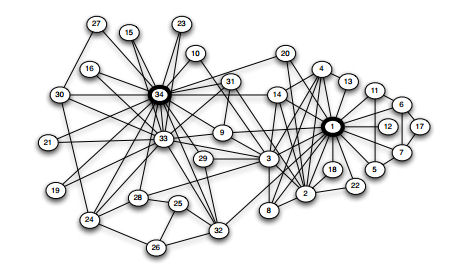
\includegraphics[scale=1]{images/17_karate_club.jpg}
\label{karate}
\caption{Relations amicales dans un club de karaté}
\end{figure}

	\item \textbf{Figure 1.2} Des employés dans un laboratoire de recherche (nœud) ont des liens entre eux :
Lignes claires = communication e-mail.
Lignes foncées = hiérarchie, organisation du laboratoire.
On voit que la communication entre les gens suit relativement bien la structure hiérarchique, mais pas complètement. On peut voir comment les gens collaborent, leurs degrés de collaboration, etc. \\

	\item \textbf{Figure 1.3} On constate que dans cette illustration, il y a beaucoup plus de nœuds. Chaque nœud est une institution financière (banque par exemple). Chaque nœud a un chemin vers un autre nœud (il y a des liens entre toutes les banques). Le centre est très dense, ça montre une faiblesse du système financier : si une banque dans le centre fait faillite par exemple, toutes les autres banques liées à elle sont également mises en danger . Donc si le noyau central est trop grand, c'est une faiblesse. En regardant cette structure, on peut trouver les faiblesses et les comprendre. Ça peut être très important.\\

	\item \textbf{Figure 1.4} Un nœud représente un blog politique et un lien, une référence vers un autre blog. Nous avons deux partis qui représentent chacun un noyau : les démocrates et les républicains. On constate qu'il y a moins de connexions entre les deux noyaux qu'à l'intérieur de ceux-ci. On peut visualiser cette structure et se poser des questions : est-ce que ce monde bipolaire est un problème ?\\\
\end{itemize}

Ce sont divers exemples que nous allons essayer d'analyser. Sur Internet, il y a beaucoup de nœuds avec de grandes capacités de calcul et de stockage. On peut maintenant regarder ces structures (pas avant). 
\section{Introduction}
\begin{itemize}
\item Structure des réseaux (Facebook, Twitter, réseau économique,...).
\item Comportement des participants (interactions : chaque nœud sera un participant et va interagir).En principe, chaque nœud ne voit que son voisinage et interagit en conséquence.
\begin{itemize}


	\item Interactions LOCALES avec conséquence GLOBALES.
	Il faut faire le lien entre ces deux choses.
	\item Effets non attendus. Ex: réseaux routiers (nœud = automobilistes, lien = routes) : \\
	S'il y a des bouchons, on augmente la capacité du réseau (ajouter une voie par exemple)
	Le résultat peut être non intuitif, ça peut être :
	\begin{itemize} 
		\item Une réduction des transferts.
		\item Une augmentation du trafic. (résultat opposé à celui attendu)
	\end{itemize}	
	\item Le \textbf{Paradoxe de Braess} nous dit que l'ajout d'une nouvelle capacité à un réseau peut réduire la performance globale (effet non attendu).
Il faut donc comprendre comment le réseau fonctionne au lieu de faire n'importe quoi et avoir des effets non attendus.
\end{itemize}
\end{itemize}
\section{Nouvelle discipline}
Les graphes et leurs propriétés évoluent avec le temps, ce n'est pas statique.\\
$\Rightarrow$Nouvelles disciplines pour analyser des graphes YouTube, Flicker, etc.\\
Synthèse de 3 disciplines :
\begin{enumerate}

	\item La théorie des graphes => mathématique
	\item La théorie des jeux => mathématique
		Exemple : YouTube impose ses règles et ceux qui utilisent YouTube sont des joueurs.
	\item La sociologie (étude des groupes sociaux): les participants sont humains ou guidés par un humain. Il n'est pas uniquement question de mathématiques, il faut aussi comprendre les humains.\\
\end{enumerate}
Dans ce cours, nous nous concentrerons principalement sur la théorie des graphes. La théorie des jeux sera très intuitive, et nous parlerons un peu de la sociologie.
\subsection{Théorie des jeux}
On a un ensemble de participants qui jouent à "un jeu" (un ensemble de règles suivies par tous les participants). Chaque participant doit agir : 
\begin{itemize}

\item Simple à spécifier (comme les échecs : 2 participants et 1 action en alternance). 
\item Compliqué : pas d'alternance, tout le monde agit en même temps. C'est un système concurrent.
\end{itemize}
Exemple d'action simple : la vente aux enchères : 
	n participants,
	règles simples (différentes techniques) \\
	
On va rester intuitif sur ce sujet, mais si on veut être plus précis, il y a des mathématiques pour ça.
\begin{itemize}

\item \textbf{Figure 1.8} Réseau d'interaction économique entre pays. Structure de l'économie mondiale : Hong Kong a un gros avantage, il a une porte d'entrée vers la Chine (à l'époque). Certains pays sont des partenaires privilégie des États-Unis... 
\item \textbf{Figure 1.9} Chemins de commerces médiévaux en Europe. L'endroit comporte des avantages : la position dans le graphe. On a toute une série d'avantages qui viennent de la structure du réseau (le comportement d'un participant peut dépendre de la structure). Si on est malin et qu'on comprend le réseau dans lequel on est, on peut essayer de se mettre dans une structure ou on a plus de pouvoir. 
\end{itemize}
Si on connaît la structure, une petite action peut suffire pour arrêter une épidémie.

\subsection{Théorie des graphes}
\subsubsection{Définitions\\}
Graphe G = ensemble de liens et de nœuds. Un lien est une paire de deux nœuds.
\begin{center}
\textbf{
G = (N,E)\\
N = nœud\\
E = edge (lien, arête)\\
}
\end{center}
Deux types de graphes :
\begin{itemize}

\item \textbf{Les graphes orientés} (avec flèches et principe de direction). Une arête/lien est une paire de nœuds. L'ordre a de l'importance. Dans cet exemple, les paires de nœuds sont : (A,B), (A,C), (D,A) et (C,D). 
\begin{figure}[!h]
\centering
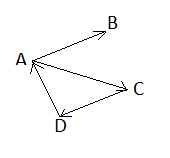
\includegraphics[scale=1]{images/17_oriente.png}
\caption{Graphe orienté}
\end{figure}
\item \textbf{Les graphes non orientés} (sans flèche, sans direction). Une arête est un ensemble de deux nœuds. On ne parle pas de "paire" vu que l'ordre des nœuds n'a pas d'importance. Ici, parler de l'arête (A,B) ou (B,A) revient à la même chose.
\begin{figure}[!h]
\centering
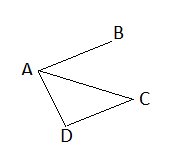
\includegraphics[scale=1]{images/17_non-oriente.png}
\caption{Graphe non orienté}
\end{figure}
\\
\end{itemize}
Dans le cours, on aura surtout affaire à des graphes non orientés.

\subsubsection{Notions de chemins et de connectivité}
\begin{itemize}

\item \textbf{Chemin} : séquence (un ordre) de nœud. Chaque paire consécutive est une arête. Un chemin peut passer plusieurs fois par la même arête (boucle), ce qui n'est pas toujours ce qu'on veut.
\item \textbf{Chemin simple} : chaque nœud est au maximum une fois dans la séquence. On ne peut plus faire le tour plusieurs fois.
\item \textbf{Cycle} : chemin qui arrive au même endroit d'où il est parti. 
	\begin{itemize}
			
	\item Le premier et le dernier nœud sont les mêmes. 
	\item Le chemin a au moins 3 liens (puisqu'on ne peut pas passer plusieurs fois par la même 	arête). 

\end{itemize}
\end{itemize}
  \newpage
  \chapter{Théorie des Graphes}


\section{Chemins et connectivité}
Nous allons commencer par rappeler la notion de chemin:
	\begin{description}
	\item[Chemin]: c'est une séquence de n\oe uds dont chaque paire consécutive est une arrête.
    \item[Chemin simple]: c'est un chemin dont chaque n\oe ud se trouve au maximum une fois dans la séquence de n\oe uds.
    \item[Cycle]: c'est un chemin dont le premier et le dernier n\oe ud sont les mêmes. Un cycle possède au moins 3 liens (arêtes).\\
	\end{description}

Maintenant, nous allons définir la notion de connectivité d'un graphe.
	\begin{description}
    \item[Connectivité]: un graphe est dit connexe si pour toutes paires de n\oe uds A et B, il existe au moins un chemin de A vers B.\\
	\end{description}

Tous les graphes ne sont en effet pas connexes. La figure \ref{graphe_non_connexe} montre un exemple de graphe non connexe.
	\begin{figure}
	\center
	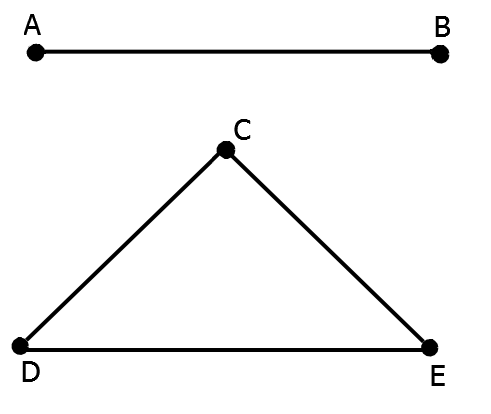
\includegraphics[scale=0.3]{images/18_graphe_non_connexe.png}
	\caption{\label{graphe_non_connexe} Graphe non connexe}
	\end{figure}
Ce graphe possède deux composants, $AB$ et $CDE$. Ces composants (qui sont maximaux) sont les parties connexes du graphe. On a les définitions suivantes:
	\begin{description}
    \item[Composant d'un graphe]: c'est un sous-graphe (partie de graphe) qui est connexe. Il est maximal s'il ne fait pas partie d'un composant plus grand.
    \item[Composant géant] : il s'agit d'un composant qui contient une fraction significative de l'ensemble des n\oe uds contenus dans le graphe.
    \end{description}
    
    Par exemple, le graphe des amitiés mondiales n'est sûrement pas connexe. En effet, il peut y avoir des habitants d'une île reculée qui se connaissent entre eux, mais qui n'ont pas de connexion avec le reste du monde. Cependant, la majorité du monde est connectée; on a donc un énorme composant géant.\\
    
    C'est une propriété générale des grands graphes complexes: il est rare qu'ils soient connexes, mais ils ont très souvent un composant géant. Avoir plusieurs composants géants est instable: il arrive vite qu'un lien se forme entre les deux composants, formant ainsi un seul composant géant. Si avant le \textsc{xv}\textsuperscript{ème} siècle, il y avait un composant géant eurasien et un autre Américain, il n'a fallu qu'un lien (la découverte de l'Amérique par Christophe Colomb) pour assembler les deux composants, avec toutes les conséquences que cela a entraîné (maladies, exploitation, etc.).\\
    
Avec les éléments que nous venons de définir, on est en mesure d'analyser tout un graphe. On peut le partitionner en composants et regarder la structure interne de chacun d'entre eux. Par exemple, dans la figure \ref{gr_connexe}, on peut partitionner en deux composantes, $ABC$ et $DEF$. On constate que le lien $CD$ est un lien spécial, car si on l'enlève, il déconnecte de graphe.\\
	\begin{figure}
	\center
	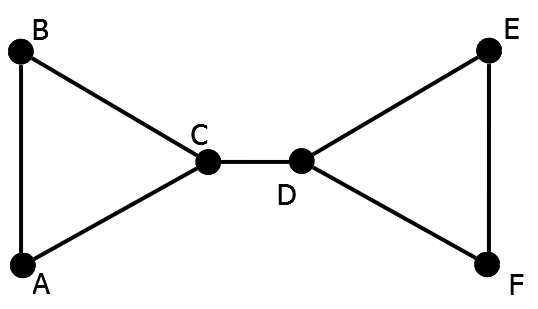
\includegraphics[scale=0.3]{images/18_gr_connexe.png}
	\caption{\label{gr_connexe} Graphe connexe}
	\end{figure}

\section{Distance entre n\oe uds}
Nous allons maintenant définir la longueur d'un chemin ainsi que la distance entre deux n\oe uds :
\begin{description}
\item[Longueur d'un chemin] : le nombre d'arêtes consécutives sur ce chemin.
\item [Distance entre 2 n\oe uds] : le chemin le plus court entre ces deux n\oe uds.
\end{description}

La méthode de calcul de distance entre deux n\oe uds est la traversée en largeur d'abord (\emph{breadth-first traversal}). Cela consiste à débuter par un n\oe ud, puis à regarder tous les n\oe uds qui sont à une distance de 1 du n\oe ud de départ. À partir de tous ceux-là, on regarde les n\oe uds qui sont à une distance 1, et donc à une distance 2 du n\oe ud de départ. On continue jusqu'à arriver au n\oe ud d'arrivée. On a donc, à chaque étape, constitué des couches de n\oe uds se trouvant à une certaine distance. Cet algorithme sera expliqué plus en détail par après.\\

\section{Phénomène du petit monde}
Le « phénomène du petit monde », aussi connu sous le vocable « paradoxe de Milgram » (du nom du psychosociologue  \textit{Stanley Milgram}), est l'hypothèse que chacun puisse être relié à n'importe quel autre individu par une courte chaîne de relations sociales. La figure \ref{petit_monde} montre la probabilité qu'ont deux personnes d'être reliés par $x$ intermédiaires. 
	\begin{figure}
	\center
	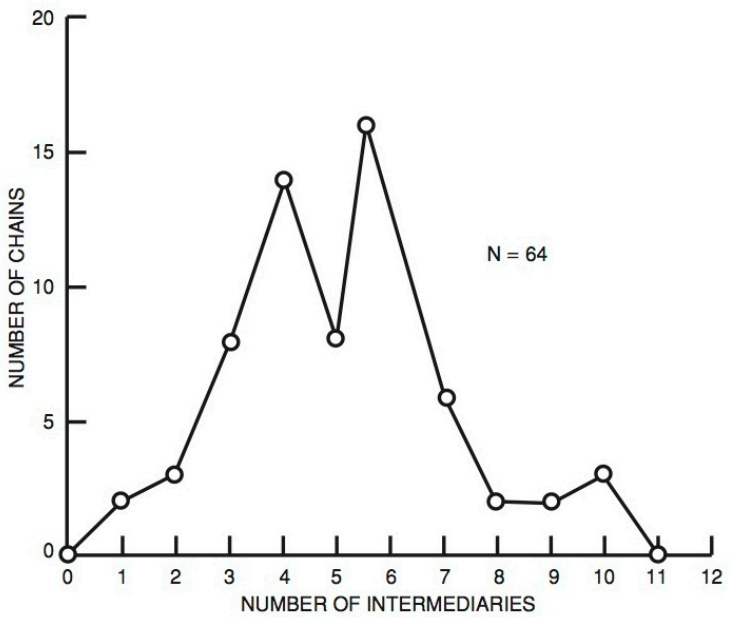
\includegraphics[scale=1]{images/18_fig.png}
	\caption{\label{petit_monde} Statistiques du phénomène du petit monde}
	\end{figure}
Cette  courte chaîne de relations sociales a été approfondie par la théorie des « six degrés de séparation » affirmant qu'en prenant deux personnes, il est possible de trouver une chaîne d'amis entre eux de taille maximum 6.
Différents types de distances entre des personnes existent, comme:
	\begin{itemize}
	\item Le nombre d'Erdos est la distance de collaboration avec le célèbre mathématicien  \textit{Paul Erdös} qui a réalisé de très nombreuses co-publications. Avoir réalisé une publication en collaboration avec Erdös correspond au nombre d'Erdös 1. Avoir écrit une publication avec quelqu'un qui a co publié avec Erdös équivaut au nombre 2, etc.
	\item Le nombre de Bacon est la distance de collaboration dans un film avec l'acteur  \textit{Kevin Bacon}.
	\end{itemize}
Ce phénomène de petit monde est particulièrement vrai pour les réseaux créés dynamiquement. Nous expliquerons plus en détail pourquoi cette affirmation est vraie dans la suite du cours.

\section{Liens forts et faibles}
Un réseau peut évoluer de différentes manières et selon différents mécanismes.
Considérons un exemple où chaque n\oe ud correspond à une personne et les arcs correspondent à un lien d'amitié (figure \ref{fermeture_triadique}).
	\begin{figure}
	\center
	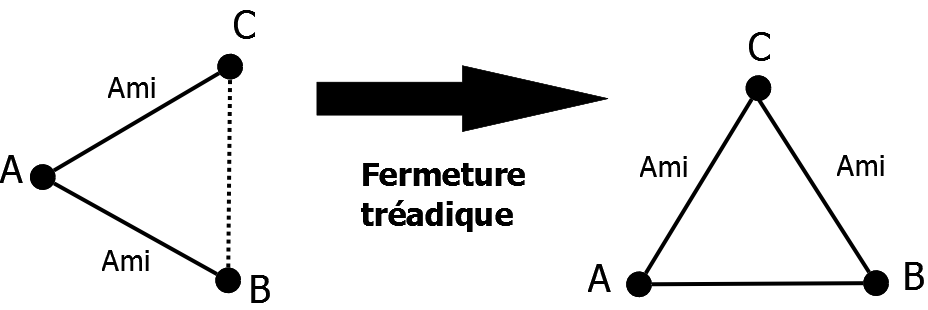
\includegraphics[scale=0.5]{images/18_fermeture_triadique.png}
	\caption{\label{fermeture_triadique} Exemple de fermeture triadique}
	\end{figure}
Dans cet exemple, on voit que $A$ est ami à la fois avec $B$ et avec $C$. Dans cette condition, il est fort probable que $B$ et $C$ deviennent eux-mêmes amis. C'est ce qu'on appelle la fermeture triadique.\\
\\
Cette situation nous amène à nous intéresser à la notion de coefficient de regroupement qui reflète la probabilité qu'un arc se crée entre deux n\oe uds dans un graphe dynamique. 
Dans l'exemple ci-dessus, cela correspondrait au fait que $C$ et $B$ deviennent amis. On peut démontrer qu'au plus on fait de fermetures triadiques, au plus le coefficient de regroupement est élevé.

\subsection*{Exemple}
Une étude a été faite dans les années 1960, par le sociologue américain \textit{Mark Granovetter}, dans laquelle il s'est intéressé aux personnes qui changent de travail et plus particulièrement à la manière dont ils trouvent un nouveau travail. Il a remarqué que les personnes trouvent du travail plutôt via des connaissances que via des amis. Cela s'explique par la structure des graphes des amis et nous amène à définir les notions de \textbf{liens forts} et de \textbf{liens faibles} (figure \ref{liens_forts_et_faibles}). La suite de cet exemple sera expliquée plus tard.\\
	\begin{figure}[!h]
	\center
	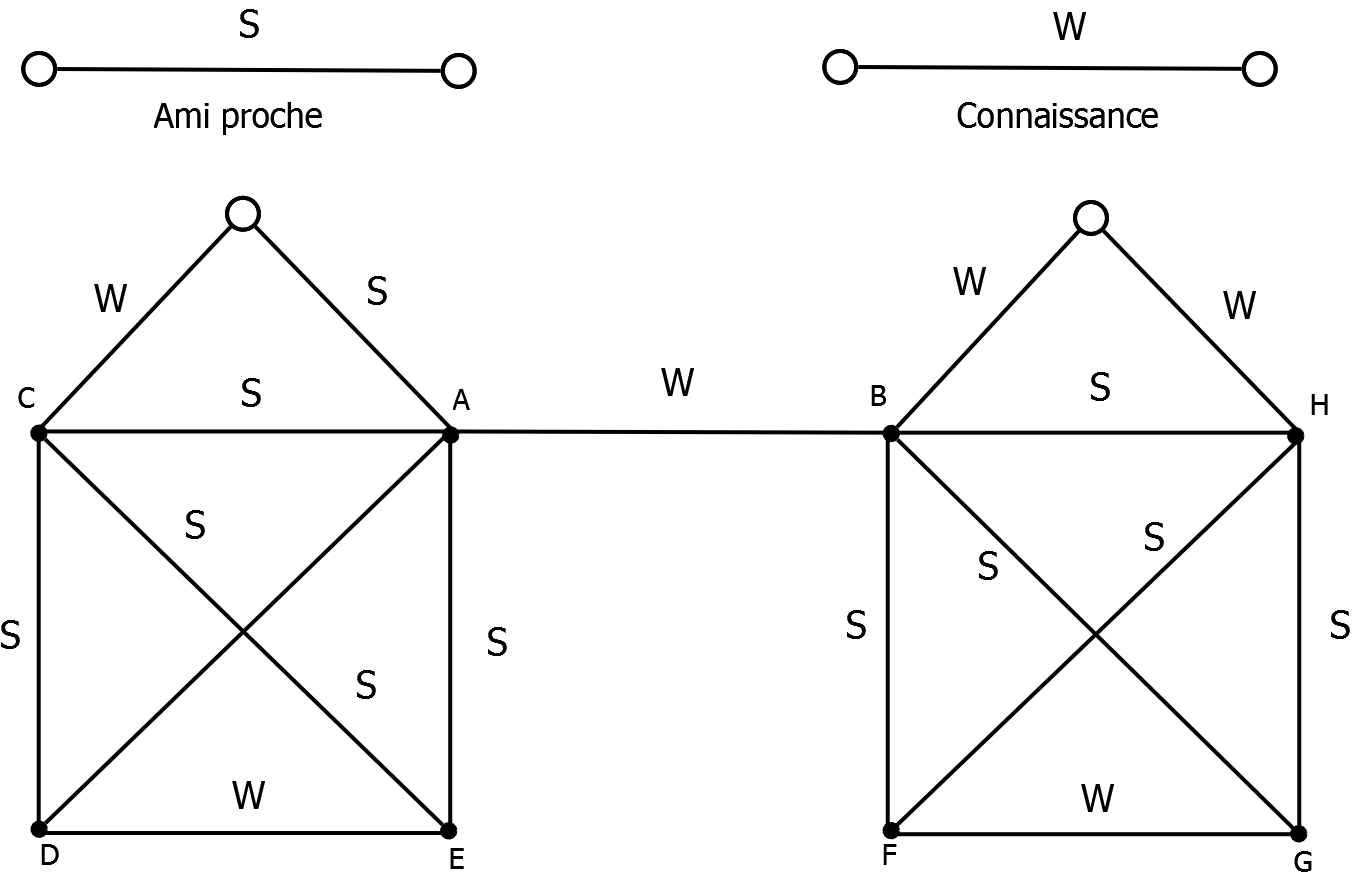
\includegraphics[scale=0.4]{images/18_liens_forts_et_faibles.png}
	\caption{\label{liens_forts_et_faibles} Liens forts et faibles}
	\end{figure}

    
\section{Ponts}
Pour expliquer l'exemple précédent, nous avons besoin de la notion de pont (figures \ref{Pont} et \ref{Pontlocal}).
	\begin{description}
	\item[Pont] Un lien entre $A$ et $B$ est un pont si l'enlèvement de ce lien aboutit à la séparation du graphe en deux composants disjoints.
    \item[Pont local] Un lien entre $A$ et $B$ est un pont local si l'enlèvement de ce lien aboutit au fait que deux composantes sont reliées par un chemin significativement plus long.
    \end{description}
    
    \begin{figure}
    \center
    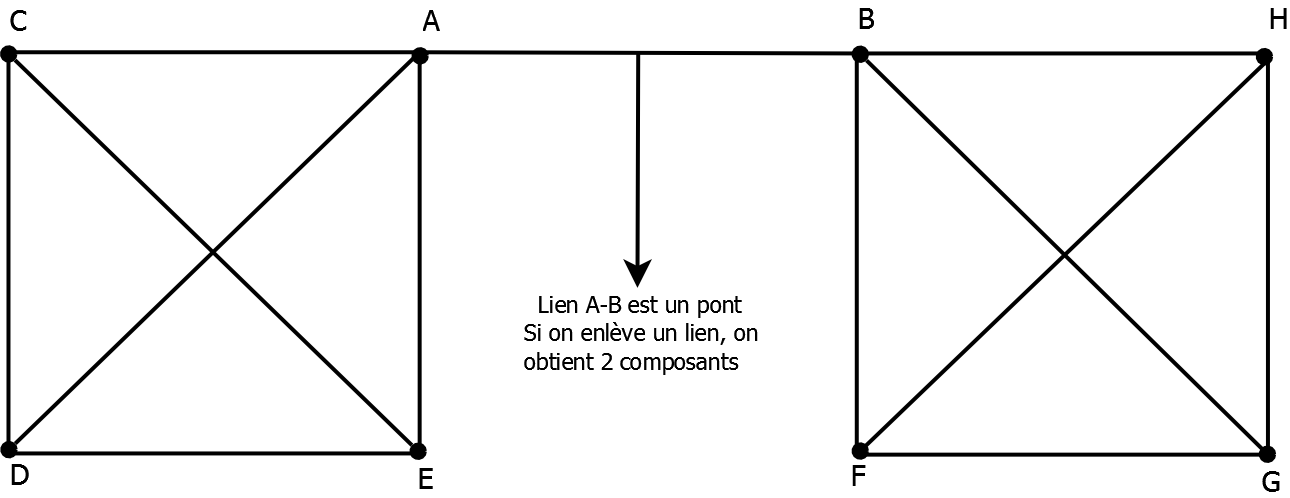
\includegraphics[scale=0.4]{images/18_Pont.png}
    \caption{\label{Pont} Pont}
    \end{figure}
    
    \begin{figure}
    \center
    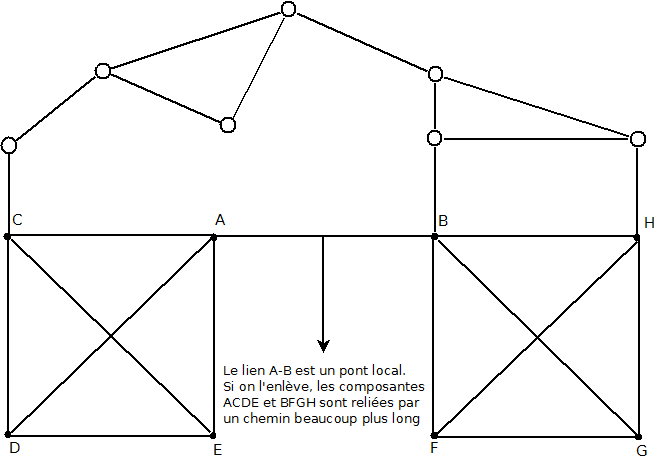
\includegraphics[scale=0.5]{images/18_Pontlocal.png}
    \caption{\label{Pontlocal} Pont local}
    \end{figure}

  \newpage
  % \section*{Conclusion}
\addcontentsline{toc}{section}{Conclusion}

Pour conclure, avec \LaTeX{} on obtient un rendu impeccable mais il faut s'investir pour le prendre en main.

  % \newpage
  \phantomsection\addcontentsline{toc}{section}{Références}
\begin{thebibliography}{ABC}	
    \bibitem[Nis]{nis} Nimal Nissanke. \emph{Introductory Logic and Sets for Computer Scientists}.
    \bibitem[LPP]{eas} David Easley and Jon Kleinberg. \emph{Networks, Crowds, and Markets: Reasoning About a Highly Connected World}.
\end{thebibliography}

\end{document}

